% !TEX root = ../OT4ML.tex

\chapter{Dynamic Optimal Transport}
\index{dynamic!optimal transport}% strictindex
\label{sec-dynamic-optimal-transport}

Optimal transport becomes especially powerful once distances between measures are seen as actions of moving mass. This chapter first develops the dynamic language: continuity equations describe admissible measure evolutions, while the Benamou--Brenier formula identifies $\Wass_2$ with a least-action principle. The path-space Schr\"odinger problem then provides its stochastic, entropy-regularized counterpart. After extending dynamic actions to other transport geometries, the chapter closes with variational mean field games, where congestion and a terminal cost turn the Benamou--Brenier action into a population-planning problem. These ideas prepare the gradient-flow and generative-model chapters that follow.
\index{continuity equation}% strictindex
\index{generative model}% strictindex
\index{Benamou-Brenier@Benamou--Brenier}% strictindex
\index{gradient!flow}% strictindex
\index{Benamou-Brenier@Benamou--Brenier!formula}% strictindex

\section{Evolutions over the Space of Measures}
\index{measure!evolution}% strictindex

We start with the continuity equation because it is the common language for particles, densities and weak measure evolutions. It also makes precise which velocity fields actually move mass.
\index{velocity field}% strictindex
\index{continuity equation}% strictindex

\paragraph{Lagrangian and Eulerian descriptions.}
\index{Lagrangian!description}% strictindex
\index{Eulerian!description}% strictindex

We consider the evolution $t \mapsto \alpha_t \in \Pp(\RR^d)$. Such an evolution can be described in a ``Lagrangian'' way as the advection of particles along a (time-dependent) vector field $v_t(x)$ in $\RR^d$. At the particle level, this advection is governed by
\index{time-dependent vector field}% strictindex
\begin{equation}
    \frac{\d x(t)}{\d t} = v_t(x(t)), \label{eq:lagrangian-advection}
\end{equation}
and we write $T_t$ for the associated flow map, so that $T_t(x(0))=x(t)$. The advected measure is then $\alpha_t = (T_t)_\sharp \alpha_0$. For discrete measures, $\alpha_t = \frac{1}{n} \sum_{i=1}^n \delta_{x_i(t)}$, meaning each $x_i(t)$ solves \eqref{eq:lagrangian-advection}.
\index{flow!map}% strictindex

In the Eulerian description, the same motion is written directly on the evolving measure: the particle ODE becomes the PDE
\index{particle ODE}% strictindex
\index{Eulerian!description}% strictindex
\begin{equation}
    \frac{\partial \alpha_t}{\partial t} + \diverg(v_t \alpha_t) = 0. \label{eq:eulerian-advection}
\end{equation}
This PDE is often referred to as the advection equation, the continuity equation, or Liouville's equation when operating over a phase space. It is only a classical PDE when $\alpha_t$ has a smooth density. For general measures, and in particular for empirical measures, it is understood in the distributional sense: for every $\varphi\in C_c^1((0,1)\times\RR^d)$,
\index{empirical!measure}% strictindex
\index{continuity equation}% strictindex
\begin{equation}\label{eq:eulerian-advection-weak}
	\int_0^1\!\int_{\RR^d}
	\left(\partial_t\varphi(t,x)+\dotp{v_t(x)}{\nabla_x\varphi(t,x)}\right)
	\d\alpha_t(x)\d t
	=
	0.
\end{equation}
This equation is obtained from~\eqref{eq:eulerian-advection} by integration by parts. Hence, for smooth positive densities, the classical and weak formulations are equivalent; the weak formulation is useful because it still makes sense for discrete measures whose particles evolve according to~\eqref{eq:lagrangian-advection}.

This interior identity provides the measure-theoretic notion of an admissible evolution. To include endpoint traces and, on a bounded domain, an impermeable boundary in the same formula, one tests up to the temporal and spatial boundaries.
\begin{defn}[Admissible continuity-equation evolution]\label{def-admissible-continuity-evolution}
\index{continuity equation!admissible evolution}% strictindex
Let $\Omega=\RR^d$, or let $\Omega\subset\RR^d$ be a bounded Lipschitz domain. A narrowly continuous curve $(\alpha_t)_{t\in[0,1]}$ in $\Pp(\overline\Omega)$ and a jointly Borel velocity field $v:(t,x)\mapsto v_t(x)$ are admissible between $\alpha_0$ and $\alpha_1$ if
\[
\int_0^1\!\int_{\overline\Omega}\norm{v_t(x)}^2\d\alpha_t(x)\d t<+\infty
\]
and, for every $\varphi\in C^1([0,1]\times\overline\Omega)$, with compact spatial support when $\Omega=\RR^d$,
\begin{equation}\label{eq-continuity-endpoint-no-flux}
\int_0^1\!\int_{\overline\Omega}
\left(\partial_t\varphi+\dotp{v_t}{\nabla_x\varphi}\right)\d\alpha_t\d t
+\int_{\overline\Omega}\varphi(0,\cdot)\d\alpha_0
-\int_{\overline\Omega}\varphi(1,\cdot)\d\alpha_1=0.
\end{equation}
On a bounded domain, allowing test functions that do not vanish on $\partial\Omega$ encodes the zero-normal-flux condition $(\alpha_t v_t)\cdot n=0$ weakly.
\end{defn}

\begin{prop}[Lagrangian flows solve the continuity equation]\label{prop-lagrangian-flow-continuity}
\index{Lagrangian!flow}% strictindex
\index{continuity equation}% strictindex
	Let $(T_t)_{t\in[0,1]}$ be a $C^1$ family of diffeomorphisms of $\RR^d$ and define $\alpha_t=(T_t)_\sharp\alpha_0$. Assume that the derivatives below are integrable with respect to $\alpha_0$, and define the Eulerian velocity field by
\index{velocity field}% strictindex
\index{Eulerian!velocity}% strictindex
	\[
		v_t(T_t(y))=\partial_t T_t(y).
	\]
	Then $(\alpha_t,v_t)$ solves the continuity equation in the weak sense~\eqref{eq:eulerian-advection-weak}.
	In particular, if $\alpha_0=\frac1n\sum_i\delta_{x_i(0)}$ is empirical, then $\alpha_t=\frac1n\sum_i\delta_{x_i(t)}$ is empirical as well, with particle velocities $\dot x_i(t)=v_t(x_i(t))$.
\end{prop}

\begin{proof}
	Let $\varphi\in C_c^1((0,1)\times\RR^d)$. Since $\alpha_t=(T_t)_\sharp\alpha_0$,
	\[
		\frac{\d}{\d t}\int \varphi(t,x)\d\alpha_t(x)
		=
		\frac{\d}{\d t}\int \varphi(t,T_t(y))\d\alpha_0(y).
	\]
	The chain rule gives
	\[
		\frac{\d}{\d t}\int \varphi(t,T_t(y))\d\alpha_0(y)
		=
		\int
		\left(
			\partial_t\varphi(t,T_t(y))
			+\dotp{\nabla_x\varphi(t,T_t(y))}{\partial_t T_t(y)}
		\right)
		\d\alpha_0(y).
	\]
	Using the definition of $v_t$ and the push-forward relation, this equals
\index{push-forward}% strictindex
	\[
		\int
		\left(
			\partial_t\varphi(t,x)+\dotp{\nabla_x\varphi(t,x)}{v_t(x)}
		\right)
		\d\alpha_t(x).
	\]
	Integrating in time and using the boundary values of $\varphi$ gives~\eqref{eq:eulerian-advection-weak}.
\end{proof}

\paragraph{From measure evolutions to vector fields.}
\index{measure!evolution}% strictindex

For a given evolution $(\alpha_t)_t$, there are typically infinitely many velocity fields $v_t$ satisfying
\index{velocity field}% strictindex
\begin{equation}\label{eq:inverse-flow}
	\partial_t\alpha_t+\diverg(\alpha_t v_t)=0.
\end{equation}
This non-uniqueness comes from the kernel of the weighted divergence. The linear space of vector fields that leave a measure $\alpha$ invariant is
\[
	\Hh_\alpha=\enscond{v\in L^2(\alpha;\RR^d)}{\diverg(\alpha v)=0\ \text{in distributions}}.
\]
It is usually non-trivial: for instance, if $\alpha$ is an isotropic Gaussian, $\Hh_\alpha$ contains rotational vector fields generated by anti-symmetric matrices.

\paragraph{Dacorogna--Moser inversion.}
\index{Dacorogna-Moser@Dacorogna--Moser!inversion}% strictindex
\index{Dacorogna-Moser@Dacorogna--Moser!construction}% strictindex

Reconstructing particles from an observed density evolution is therefore ill-posed. For a smooth positive density $\alpha_t=\rho_t\,\d x$, a simple choice, introduced by Dacorogna and Moser~\cite{DacorognaMoser1990}, is to impose that the flux $\rho_t v_t$ is a gradient field. With a fixed convention for the inverse Laplacian, this gives formally
\index{flux}% strictindex
\begin{equation}\label{eq:dacorogna-moser}
	v_t=-\frac{1}{\rho_t}\nabla\Delta^{-1}(\partial_t\rho_t),
\end{equation}
with suitable boundary conditions, for instance vanishing at infinity. This formula is useful conceptually but delicate when $\rho_t$ vanishes, and it does not generally produce a gradient velocity field.
\index{velocity field}% strictindex
\index{gradient!velocity}% strictindex

The classical Dacorogna--Moser construction uses the linear density path. If $\alpha_i=\rho_i\,\d x$ are smooth positive densities with the same total mass on a bounded connected domain $\Omega$, set
\[
	\alpha_t=(1-t)\alpha_0+t\alpha_1=\rho_t\,\d x,
	\qquad
	\rho_t=(1-t)\rho_0+t\rho_1.
\]
Choose a time-independent flux $w$ satisfying
\[
	\diverg w=\rho_0-\rho_1,
	\qquad
	w\cdot n=0\quad\hbox{on }\partial\Omega,
\]
for instance $w=-\nabla\phi$ with $\Delta\phi=\rho_1-\rho_0$ and Neumann boundary condition. Then
\[
	v_t=\frac{w}{\rho_t}
\]
satisfies $\partial_t\rho_t+\diverg(\rho_t v_t)=0$. The flow
$\partial_t T_t=v_t\circ T_t$, $T_0=\Id$, therefore transports
$\rho_0\d x$ onto $\rho_t\d x$, and $T_1$ solves the prescribed-Jacobian problem
$\rho_1(T_1(x))\det(\nabla T_1(x))=\rho_0(x)$.

\paragraph{Least-square inversion and gradient structure.}
\index{least squares!inversion}% strictindex
\index{gradient!structure}% strictindex

A more robust choice, used implicitly in flow matching, optimal transport and Wasserstein gradient flows, is to select among all admissible velocities the one with smallest kinetic energy:
\index{Wasserstein!gradient}% strictindex
\index{gradient!flow}% strictindex
\index{Wasserstein!gradient flow}% strictindex
\index{flow matching}% strictindex
\begin{equation}\label{eq:least-square-field}
	\umin{v}
	\frac12\int_0^1\!\int_{\RR^d}\norm{v_t(x)}^2\,\d\alpha_t(x)\d t
	\quad
	\text{subject to}
	\quad
	\partial_t\alpha_t+\diverg(\alpha_t v_t)=0.
\end{equation}

\begin{prop}[Least-square velocities are gradients]\label{prop-least-square-gradient-velocity}
\index{least squares!velocity}% strictindex
\index{gradient!velocity}% strictindex
	Assume that $\alpha_t=\rho_t\,\d x$ is a smooth positive density curve, that $\partial_t\rho_t$ has zero integral, and that boundary terms vanish. The minimizer of~\eqref{eq:least-square-field}, if it exists, is a gradient field
	\[
		v_t=\nabla\phi_t,
	\]
	where $\phi_t$, unique up to an additive constant on each connected component, solves the weighted Poisson equation
\index{weighted!Poisson equation}% strictindex
	\begin{equation}\label{eq:least-square-field-explicit}
		-\diverg(\rho_t\nabla\phi_t)=\partial_t\rho_t,
		\qquad
		v_t=-\nabla\Delta_{\alpha_t}^{-1}(\partial_t\alpha_t),
		\quad
		\Delta_{\alpha_t}\phi=\diverg(\alpha_t\nabla\phi).
	\end{equation}
\end{prop}

\begin{proof}
	Introduce a Lagrange multiplier $\phi_t$ for the continuity equation. The constrained problem has the formal saddle formulation
\index{continuity equation}% strictindex
	\[
		\umin{v}\umax{\phi}
		\int_0^1
		\left[
			\frac12\int_{\RR^d}\norm{v_t(x)}^2\,\d\alpha_t(x)
			+\int_{\RR^d}\phi_t(x)\big(\diverg(\alpha_t v_t)(x)+\partial_t\alpha_t(x)\big)\d x
		\right]\d t.
	\]
	Integrating by parts in the divergence term gives, for each $t$,
	\[
		\int \left(\frac12\norm{v_t}^2-\dotp{\nabla\phi_t}{v_t}\right)\d\alpha_t
		+
		\int \phi_t\,\partial_t\alpha_t.
	\]
	The pointwise minimizer in $v_t$ is therefore $v_t=\nabla\phi_t$. Substituting this into the constraint $\partial_t\rho_t+\diverg(\rho_t v_t)=0$ gives the weighted Poisson equation in~\eqref{eq:least-square-field-explicit}. The inverse notation is just a shorthand for solving this equation on zero-mean right-hand sides, modulo additive constants.
\index{zero mean}% strictindex
\index{weighted!Poisson equation}% strictindex
\end{proof}

In general this inversion is still computationally demanding, but special choices of $(\alpha_t)_t$ lead to simpler formulas; this is the mechanism exploited later by flow matching in Section~\ref{sec-generative-flow-matching}.
\index{flow matching}% strictindex

\section{Benamou--Brenier Dynamic Formulation of OT}
\index{Benamou-Brenier@Benamou--Brenier}% strictindex
\index{Benamou-Brenier@Benamou--Brenier!formulation}% strictindex
\index{Benamou-Brenier@Benamou--Brenier!formula}% strictindex
\label{sec-benamou-brenier-dynamic}

The dynamic formulation identifies $\Wass_2$ with the kinetic energy of the cheapest continuity-equation path. It is the point where OT becomes a least-action principle.
\index{continuity equation}% strictindex
\index{dynamic!formulation}% strictindex

\paragraph{Benamou--Brenier formulation.}

Instead of assuming that a whole curve $(\alpha_t)_{t\in[0,1]}$ is prescribed, one only fixes its endpoints $\alpha_0$ and $\alpha_1$ and minimizes the least-square energy~\eqref{eq:least-square-field}. The theorem of Benamou and Brenier states that this geodesic energy is exactly the squared Wasserstein distance~\cite{benamou2000computational}.
\index{Wasserstein!distance}% strictindex

The kinetic energy of an admissible evolution is the basic dynamic action.
\begin{defn}[Benamou--Brenier action]\label{def-benamou-brenier-action}
For an admissible pair $(\alpha_t,v_t)$, define
\[
\operatorname{Act}_2(\alpha,v)
\eqdef
\int_0^1\!\int_{\RR^d}\norm{v_t(x)}^2\d\alpha_t(x)\d t.
\]
\end{defn}

\begin{thm}[Benamou--Brenier]\label{thm-benamou-brenier}
\index{Benamou-Brenier@Benamou--Brenier}% strictindex
	For probability measures $\alpha_0,\alpha_1\in\Pp_2(\RR^d)$,
\index{probability measure}% strictindex
	\begin{equation}\label{eq:benamou-brenier}
	\Wass_2^2(\alpha_0,\alpha_1)
	=
	\inf_{(\alpha_t,v_t)}
	\int_0^1\!\int_{\RR^d}\norm{v_t(x)}^2\,\d\alpha_t(x)\d t,
	\end{equation}
	where the infimum is over $(\alpha_t,v_t)$ solving $\partial_t\alpha_t+\nabla\!\cdot(\alpha_t v_t)=0$ with $\alpha_{t=0}=\alpha_0$ and $\alpha_{t=1}=\alpha_1$. If $\alpha_0$ has a density and $T$ is the optimal Monge map $T_\sharp\alpha_0=\alpha_1$, a minimizing curve is
\index{Monge!problem}% strictindex
	\begin{equation}\label{eq:static-to-dynamic}
		\alpha_t=((1-t)\Id+tT)_\sharp\alpha_0,
		\qquad
		v_t\big((1-t)x+tT(x)\big)=T(x)-x
		\quad\text{for $\alpha_0$-a.e.\ $x$ and a.e.\ $t\in(0,1)$}.
	\end{equation}
\end{thm}

\begin{proof}
	For the inequality ``dynamic $\leq$ static'', assume first that a Monge map $T$ exists and define $(\alpha_t,v_t)$ by~\eqref{eq:static-to-dynamic}. Since the Lagrangian velocity $T(x)-x$ is independent of $t$,
\index{Monge!problem}% strictindex
	\[
		\int_0^1\!\int\norm{v_t}^2\,\d\alpha_t\d t
		=
		\int\norm{T(x)-x}^2\,\d\alpha_0(x),
	\]
	so the dynamic cost is no larger than the static Monge cost. Without a Monge map, the same construction is made with an optimal coupling $\pi$: sample $(X,Y)\sim\pi$ and move along the straight path $\gamma_{X,Y}(t)=(1-t)X+tY$. This path measure has action $\int\norm{x-y}^2\d\pi(x,y)$; projecting path velocities onto their conditional mean at time $t$ gives an admissible Eulerian velocity with no larger action, so the dynamic value is no larger than the Kantorovich value.
\index{dynamic!value}% strictindex
\index{optimal coupling}% strictindex
\index{Eulerian!velocity}% strictindex
\index{path measure}% strictindex

	Conversely, for a smooth deterministic path, take the flow $T_t$ defined by $\dot T_t=v_t\circ T_t$ and $T_0=\Id$. Then $\alpha_t=(T_t)_\sharp\alpha_0$ and $(T_1)_\sharp\alpha_0=\alpha_1$. Jensen's inequality gives
\index{Jensen inequality}% strictindex
	\[
		\norm{T_1(x)-x}^2
		\leq
		\int_0^1\norm{v_t(T_t(x))}^2\d t.
	\]
	After integration with respect to $\alpha_0$, the Monge cost is bounded above by the dynamic action. For general finite-energy solutions of the continuity equation, the superposition principle lifts the curve to a probability measure on absolutely continuous paths; applying Jensen's inequality pathwise gives a coupling of the endpoints whose quadratic cost is no larger than the action. Thus the Kantorovich value is bounded above by the dynamic value.
\index{dynamic!value}% strictindex
\index{absolutely continuous path}% strictindex
\index{dynamic!action}% strictindex
\index{superposition principle}% strictindex
\index{Jensen inequality}% strictindex
\index{probability measure}% strictindex
\index{continuity equation}% strictindex
\index{quadratic!cost}% strictindex
\end{proof}

\paragraph{Convex momentum-based reformulation.}
\index{momentum formulation}% strictindex

Although~\eqref{eq:benamou-brenier} is not jointly convex in $(\alpha_t,v_t)$, it becomes convex after replacing velocities by momenta. Given a velocity \(v\in L^2(\alpha;\RR^d)\), define the momentum
\[
	\omega\eqdef \alpha v,
	\qquad
	\omega(A)=\int_A v(x)\,\d\alpha(x),
\]
which is a finite \(\RR^d\)-valued measure. The nonlinear relation \(\omega=\alpha v\) is eliminated by the following measure perspective.
\begin{defn}[Quadratic perspective action]\label{def-quadratic-perspective-action}
\begin{equation}\label{eq-quadratic-perspective}
	J(a,m)
	\eqdef
	\begin{cases}
		\norm{m}^2/a, & a>0,\\
		0, & a=0\ \text{and}\ m=0,\\
	+\infty, & a=0\ \text{and}\ m\neq0,
	\end{cases}
	\qquad
	(a,m)\in[0,+\infty)\times\RR^d.
\end{equation}
\index{perspective function}% strictindex
\index{quadratic!perspective}% strictindex
If \(\lambda\) dominates \(\alpha\) and \(|\omega|\), define
\begin{equation}\label{eq-measure-perspective-action}
	\mathbb J(\alpha,\omega)
	\eqdef
	\int
	J\left(
		\frac{\d\alpha}{\d\lambda}(x),
		\frac{\d \omega}{\d\lambda}(x)
	\right)\d\lambda(x).
\end{equation}
\end{defn}
\index{perspective function}% strictindex
\index{quadratic!perspective}% strictindex
The pointwise function is lower-semicontinuous, convex and positively \(1\)-homogeneous: \(J(\eta a,\eta m)=\eta J(a,m)\) for \(\eta\geq0\).
The definition is independent of the dominating measure \(\lambda\): after replacing \(\lambda\) by another dominating measure, both Radon--Nikodym densities are rescaled by the same factor, which cancels with the change of reference measure by the \(1\)-homogeneity of \(J\). Equivalently, this is the standard integral functional associated with a convex normal integrand, used in the measure-valued relaxation of dynamic OT~\cite{ambrosio2006gradient}; see also Rockafellar's perspective construction~\cite{rockafellar2015convex}. In particular,
\[
	\mathbb J(\alpha,\omega)<+\infty
	\quad\Longleftrightarrow\quad
	\omega=v\alpha\ \text{with}\ v\in L^2(\alpha;\RR^d),
	\qquad
	\mathbb J(\alpha,\omega)=\int\norm{v}^2\,\d\alpha.
\]

The Benamou--Brenier problem can now be written with the linear continuity equation in the pair \((\alpha_t,\omega_t)\):
\index{perspective function}% strictindex
\index{momentum}% strictindex
\index{Benamou-Brenier@Benamou--Brenier}% strictindex
\begin{equation}\label{eq:benamou-brenier-convex}
	\Wass_2^2(\alpha_0,\alpha_1)
	=
	\inf_{\substack{\partial_t\alpha_t+\diverg \omega_t=0\\
	\alpha_{t=0}=\alpha_0,\ \alpha_{t=1}=\alpha_1}}
	\int_0^1 \mathbb J(\alpha_t,\omega_t)\,\d t.
\end{equation}
In the absolutely continuous case \(\alpha_t=\rho_t\,\d x\) and \(\omega_t=m_t\,\d x\), this becomes
\[
	\inf_{\substack{\partial_t\rho_t+\diverg m_t=0\\
	\rho_{t=0}\d x=\alpha_0,\ \rho_{t=1}\d x=\alpha_1}}
	\int_0^1\!\int_{\RR^d}
	J(\rho_t(x),m_t(x))\,\d x\,\d t
	=
	\inf_{\substack{\partial_t\rho_t+\diverg m_t=0\\
	\rho_{t=0}\d x=\alpha_0,\ \rho_{t=1}\d x=\alpha_1}}
	\int_0^1\!\int_{\RR^d}
	\frac{\norm{m_t(x)}^2}{\rho_t(x)}\,\d x\,\d t,
\]
with the conventions encoded in~\eqref{eq-quadratic-perspective}. This convex reformulation enables geodesic interpolation by convex optimization once the domain is discretized.
\index{recession convention}% strictindex
\index{momentum}% strictindex

\paragraph{Dual Hamilton--Jacobi formulation.}
\index{Hamilton-Jacobi@Hamilton--Jacobi equation}% strictindex
\index{Benamou-Brenier@Benamou--Brenier!dual}% strictindex

The momentum formulation also has a useful dual. It turns the least-action problem into a Hamilton--Jacobi subsolution inequality for a scalar potential, with equality on the part of space-time actually visited by the optimal curve. This is the dual dynamic formulation already present in the original Benamou--Brenier perspective~\cite{benamou2000computational}; see also the standard accounts~\cite{Villani03,SantambrogioBook}. The constants below follow the convention of~\eqref{eq:benamou-brenier-convex}, where the kinetic energy has no factor $1/2$.
\index{perspective function}% strictindex

\begin{prop}[Dual Benamou--Brenier problem]\label{prop-benamou-brenier-dual}
	Assume, for simplicity, that the densities are smooth, compactly supported, and that boundary terms vanish. Then the convex dynamic value~\eqref{eq:benamou-brenier-convex} has the dual formulation
	\begin{equation}\label{eq:benamou-brenier-dual}
		\Wass_2^2(\alpha_0,\alpha_1)
		=
		\sup_{\phi}
		\enscond{
		\int_{\RR^d}\phi_1\,\d\alpha_1
		-
		\int_{\RR^d}\phi_0\,\d\alpha_0
		}{
		\partial_t\phi_t+\frac14\norm{\nabla\phi_t}^2\leq 0
		},
	\end{equation}
	where the supremum is over smooth test potentials $\phi:[0,1]\times\RR^d\to\RR$. In the general metric-measure statement, the same formula is understood after relaxation: $\phi$ is a Hamilton--Jacobi subsolution, for instance in the viscosity sense, and finite-dimensional discretizations follow directly from Fenchel--Rockafellar duality.
\index{Hamilton-Jacobi@Hamilton--Jacobi equation}% strictindex

	If $(\rho,m)$ and $\phi$ are smooth primal and dual optimizers, then
	\begin{equation}\label{eq:bb-primal-dual-relation}
		m_t=\frac{\rho_t}{2}\nabla\phi_t,
		\qquad
		\partial_t\phi_t+\frac14\norm{\nabla\phi_t}^2=0
		\quad\text{on }\{\rho_t>0\}.
	\end{equation}
	Equivalently, the optimal Eulerian velocity is $v_t=m_t/\rho_t=\nabla\phi_t/2$.
\index{Eulerian!velocity}% strictindex
\end{prop}

\begin{proof}
	Let $(\rho,m)$ satisfy the continuity equation and let $\phi$ be smooth. Multiplying the constraint by $\phi$ and integrating by parts gives
\index{continuity equation}% strictindex
	\[
		\int_{\RR^d}\phi_1\,\d\alpha_1
		-
		\int_{\RR^d}\phi_0\,\d\alpha_0
		=
		\int_0^1\!\int_{\RR^d}
		\left(\rho_t\,\partial_t\phi_t+\dotp{m_t}{\nabla\phi_t}\right)\d x\d t.
	\]
	If $\partial_t\phi_t+\norm{\nabla\phi_t}^2/4\leq0$, Young's inequality yields, pointwise,
	\[
		\rho\,\partial_t\phi+\dotp{m}{\nabla\phi}
		\leq
		-\frac{\rho}{4}\norm{\nabla\phi}^2+\dotp{m}{\nabla\phi}
		\leq
		J(\rho,m),
	\]
	with the perspective convention~\eqref{eq-quadratic-perspective}. Hence the dual objective of every feasible $\phi$ is no larger than the action of every feasible primal pair.
\index{perspective function}% strictindex

	Conversely, introduce $\phi$ as a Lagrange multiplier for $\partial_t\rho+\diverg m=0$. After integration by parts, and up to the fixed endpoint contribution in~\eqref{eq:benamou-brenier-dual}, the pointwise minimization over $(\rho,m)$ contains
	\[
		J(\rho,m)-\rho\,\partial_t\phi-\dotp{m}{\nabla\phi}.
	\]
	For fixed $\rho>0$, its minimum over $m$ is attained at $m=\rho\nabla\phi/2$ and equals $-\rho(\partial_t\phi+\norm{\nabla\phi}^2/4)$. The recession cases in~\eqref{eq-quadratic-perspective} give the same conclusion when \(\rho=0\). Thus the infimum over $\rho\geq0$ is finite exactly when the Hamilton--Jacobi inequality holds, in which case the pointwise infimum is $0$. Fenchel--Rockafellar duality then gives no duality gap. Equality in the two pointwise inequalities gives~\eqref{eq:bb-primal-dual-relation}.
\index{Hamilton-Jacobi@Hamilton--Jacobi equation}% strictindex
\index{duality!Fenchel-Rockafellar@Fenchel--Rockafellar}% strictindex
\index{perspective function}% strictindex
\end{proof}

This also recovers the static Kantorovich inequality from a dynamic principle. If $\gamma$ is any smooth curve with $\gamma(0)=x$ and $\gamma(1)=y$, then
\[
	\frac{\d}{\d t}\phi_t(\gamma(t))
	=
	\partial_t\phi_t(\gamma(t))+\dotp{\nabla\phi_t(\gamma(t))}{\dot\gamma(t)}
	\leq
	\norm{\dot\gamma(t)}^2,
\]
where the last inequality uses $\partial_t\phi+\norm{\nabla\phi}^2/4\leq0$ and Young's inequality. Integrating and minimizing over curves gives
\[
	\phi_1(y)-\phi_0(x)\leq\norm{x-y}^2.
\]
Thus $(-\phi_0,\phi_1)$ is a feasible static Kantorovich dual pair for the quadratic cost. At optimality the inequality is saturated on the endpoint pairs connected by the primal characteristics, which is the Eulerian version of complementary slackness.
\index{Kantorovich!dual}% strictindex
\index{complementary slackness}% strictindex

Figure~\ref{fig:dynamic-benamou-brenier-duality} displays these primal--dual relations for a one-dimensional mixture transport, including the Hamilton--Jacobi contact identity along the active mass.

\begin{figure}[ht]
\centering
\begin{tabular}{@{}ccc@{}}
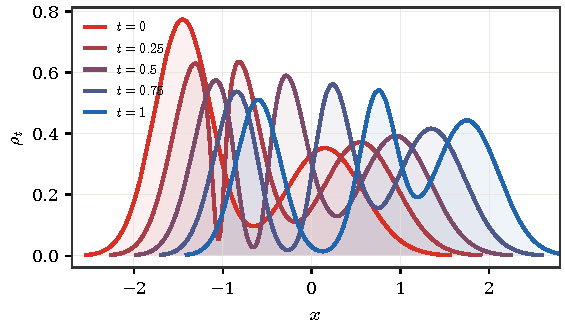
\includegraphics[width=.31\linewidth]{figures/dynamic-benamou-brenier-duality/density.pdf} &
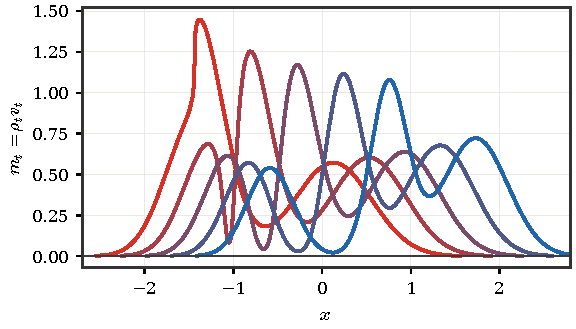
\includegraphics[width=.31\linewidth]{figures/dynamic-benamou-brenier-duality/momentum.pdf} &
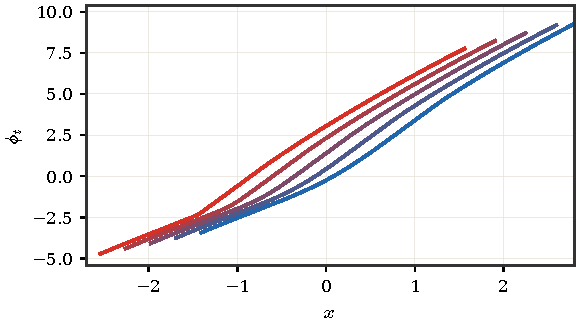
\includegraphics[width=.31\linewidth]{figures/dynamic-benamou-brenier-duality/dual-potential.pdf}
\\[-.1em]
\small density $\rho_t$ &
\small momentum density $m_t$ &
\small dual potential $\phi_t$
\end{tabular}
\caption{\emph{One-dimensional Benamou--Brenier primal and dual solutions.} The endpoints are Gaussian mixtures and the solution is computed from monotone quantile interpolation. The left and middle panels show the primal density and the momentum density $m_t=\rho_t v_t$. The right panel shows the dual Hamilton--Jacobi potential, normalized up to an additive constant. Along the active transported mass, the notebook checks the primal--dual identities $m_t=\rho_t\partial_x\phi_t/2$ and $\partial_t\phi_t+|\partial_x\phi_t|^2/4=0$.}
\index{Hamilton-Jacobi@Hamilton--Jacobi equation}% strictindex
\index{momentum}% strictindex
\label{fig:dynamic-benamou-brenier-duality}
\end{figure}

\paragraph{Proximal splitting.}
\index{proximal!splitting}% strictindex
\index{Douglas-Rachford splitting}% strictindex

The convex momentum formulation also explains the original Benamou--Brenier solver. Papadakis, Peyr\'e and Oudet~\cite{FPapPeyOud13} showed that, after discretization, the ALG2 scheme is a Douglas--Rachford splitting, equivalently ADMM on the Fenchel--Rockafellar dual. Suppressing discretization indices, write \(U=(\rho,m)\), where \(m\) is the density of the momentum measure. Using the perspective~\eqref{eq-quadratic-perspective}, set
\index{perspective function}% strictindex
\[
	\mathcal F(U)=\int_0^1\!\int_{\RR^d}J(\rho_t(x),m_t(x))\,\d x\,\d t,
	\qquad
	\mathcal C=\enscond{(\rho,m)}{\partial_t\rho+\diverg m=0,\ \rho_0\d x=\alpha_0,\ \rho_1\d x=\alpha_1},
\]
and let $\mathcal G=\iota_{\mathcal C}$ be the indicator of this affine continuity constraint. The convex Benamou--Brenier problem is therefore
\[
	\min_U\; \mathcal F(U)+\mathcal G(U).
\]
On the resulting Hilbert space of unknowns, or formally for an $L^2$-type product structure, the two proximal operators are
\index{proximal!operator}% strictindex
\[
	\prox_{\tau\mathcal F}(\bar U)
	=
	\argmin_U
	\frac12\norm{U-\bar U}_{\mathsf H}^2+\tau\mathcal F(U),
	\qquad
	\prox_{\tau\mathcal G}(\bar U)
	=
	\argmin_{U\in\mathcal C}
	\frac12\norm{U-\bar U}_{\mathsf H}^2.
\]
For the standard product metric, the first map is local in $(t,x)$: it is the proximal operator of the convex perspective $J$. The second map is the orthogonal projection onto the affine set defined by the divergence equation and endpoint constraints. Douglas--Rachford then alternates these two simple operations:
\index{proximal!operator}% strictindex
\index{Douglas-Rachford algorithm}% strictindex
\[
	\begin{aligned}
		U^{(\ell+1)} &= \prox_{\tau\mathcal F}(Z^{(\ell)}),\\
		\widetilde U^{(\ell+1)} &= \prox_{\tau\mathcal G}(2U^{(\ell+1)}-Z^{(\ell)}),\\
		Z^{(\ell+1)} &= Z^{(\ell)}+\widetilde U^{(\ell+1)}-U^{(\ell+1)}.
	\end{aligned}
\]
Equivalently one may swap the roles of $\mathcal F$ and $\mathcal G$. At convergence, the two shadow sequences $U^{(\ell)}$ and $\widetilde U^{(\ell)}$ agree and give a minimizer of the convex dynamic problem. This viewpoint is useful because it separates the nonlinear but pointwise perspective proximal step from the global but linear projection onto the continuity equation~\cite{FPapPeyOud13,Eckstein1992}.
\index{perspective function}% strictindex
\index{continuity equation}% strictindex
\index{duality!Fenchel-Rockafellar@Fenchel--Rockafellar}% strictindex
\index{ADMM}% strictindex

\begin{alg}[Douglas--Rachford for dynamic Benamou--Brenier]\label{alg:benamou-brenier-douglas-rachford}
\index{Douglas-Rachford splitting}% strictindex
\textbf{Input:} Functionals $\mathcal F,\mathcal G=\iota_{\mathcal C}$, proximal parameter $\tau>0$, initial field $Z^{(0)}$, tolerance $\mathrm{tol}>0$, iteration budget $L\geq1$.

\textbf{Output:} Discrete density-momentum field $U^\star$.

\textbf{For} $\ell=0,\ldots,L-1$ \textbf{do}:
\begin{algblock}
\(U^{(\ell+1)}=\prox_{\tau\mathcal F}(Z^{(\ell)})\).

\textbf{Project} reflected point:
\(\widetilde U^{(\ell+1)} = \prox_{\tau\mathcal G}(2U^{(\ell+1)}-Z^{(\ell)}) = \Proj_{\mathcal C}(2U^{(\ell+1)}-Z^{(\ell)})\).

\textbf{Update}
\(Z^{(\ell+1)}=Z^{(\ell)}+\widetilde U^{(\ell+1)}-U^{(\ell+1)}\).

\textbf{If} $\norm{U^{(\ell+1)}-\widetilde U^{(\ell+1)}}\leq\mathrm{tol}$ \textbf{then}:
\begin{algblock}
\textbf{Return} $U^{(\ell+1)}$.
\end{algblock}
\end{algblock}

\textbf{Return} $U^{(L)}$.
\end{alg}

Figure~\ref{fig:dynamic-benamou-brenier-geodesic} complements the Eulerian optimization viewpoint with the Lagrangian picture: matched particles travel along the straight characteristics of the minimizing curve.

\begin{figure}[ht]
\centering
\newcommand{\bbgeodesicpanelheight}{.155\linewidth}
\begin{tabular}{@{}cc@{}}

\includegraphics[height=\bbgeodesicpanelheight]{figures/dynamic-benamou-brenier-geodesic/density-sequence.pdf} &
\index{Benamou-Brenier@Benamou--Brenier}% strictindex
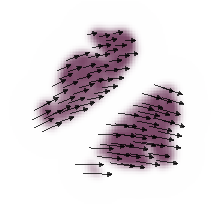
\includegraphics[height=\bbgeodesicpanelheight]{figures/dynamic-benamou-brenier-geodesic/midpoint-velocities.pdf}
\\[-.1em]
\small density sequence &
\small midpoint velocities
\end{tabular}
\caption{\emph{Benamou--Brenier geodesic between two sampled silhouettes.} A discrete quadratic OT plan between finely subsampled cat and two-disks point clouds induces the McCann interpolation $Z_t=(1-t)X+tY$, which is the Lagrangian realization of the least-action solution. The left panel renders local color images of the smaller-bandwidth kernel-smoothed densities with enough padding to include the full silhouettes. The right panel overlays shortened velocity arrows centered at evenly subsampled midpoint particles $Z_{1/2}$; each displayed arrow runs in data coordinates from a source-side tail to a target-side head along the matched characteristic direction $Y-X$, but is not drawn as the full endpoint segment from $X$ to $Y$.}
\index{McCann!interpolation}% strictindex
\label{fig:dynamic-benamou-brenier-geodesic}
\end{figure}

\paragraph{Path-space formulation.}\label{rem-bb-path-space}
\index{path-space formulation}% strictindex
	Let $\Ss=C([0,1];\RR^d)$ be the space of continuous paths endowed with the uniform topology. For $t\in[0,1]$ define the evaluation map
	\[
		e_t:\Ss\to\RR^d,
		\qquad
		e_t(\gamma)=\gamma(t).
	\]
	The Benamou--Brenier cost admits the equivalent formulation
\index{Benamou-Brenier@Benamou--Brenier}% strictindex
	\[
		\Wass_2^2(\alpha_0,\alpha_1)
		=
		\inf_{M\in\Pp(\Ss)}
		\enscond{
			\int_{\Ss}\!\int_0^1\norm{\dot\gamma(t)}^2\d t\,\d M(\gamma)
		}{
			(e_0)_\sharp M=\alpha_0,\ (e_1)_\sharp M=\alpha_1
		}.
	\]
	The inner kinetic energy is understood as $+\infty$ when $\gamma$ is not absolutely continuous. If $\alpha_0$ has a density, the minimizer $M^*$ is unique. Its time marginals reproduce the optimal curve: $\alpha_t=(e_t)_\sharp M^*$ for all $t$. Furthermore, for a.e.\ $t$, denoting $\dot e_t(\gamma)=\dot\gamma(t)$ on absolutely continuous paths, the conditional law of the velocity is deterministic:
\index{absolutely continuous path}% strictindex
\index{conditional!law}% strictindex
	\[
		(e_t,\dot e_t)_\sharp M^*(\d x,\d q)
		=
		\alpha_t(\d x)\delta_{v_t^*(x)}(\d q),
	\]
	where $v_t^*$ is the optimal velocity field in the Benamou--Brenier formulation. Hence $M^*$ concentrates on straight-line geodesics and, for a.e.\ $t$, assigns exactly one direction at $\alpha_t$-a.e.\ spatial point.
\index{Benamou-Brenier@Benamou--Brenier}% strictindex
\index{velocity field}% strictindex
\index{Benamou-Brenier@Benamou--Brenier!formulation}% strictindex

%%%%%%%%%%%%%%%%%%%%%%%%%%%%%%%%%%%%%%%%%%%%%%%%%%%%%%%%%%%%%%%%%%%%%%%%%%%

\section{Path-Space Schr\"odinger Problem}
\index{path-space formulation}% strictindex
\index{Schrodinger@Schr\"odinger!problem}% strictindex
\index{Schrodinger@Schr\"odinger!bridge}% strictindex
\label{sec-path-space-schrodinger}

The path-space formulation at the end of Section~\ref{rem-bb-path-space} recasts unregularized quadratic transport as a least-action problem over laws of trajectories. Schr\"odinger's reciprocal problem is its stochastic counterpart: a noisy reference dynamics replaces deterministic least-action paths. After optimizing out the conditional law of a trajectory given its endpoints, only the endpoint coupling remains, and the static entropic problem~\eqref{eq-entropic-generic} reappears. This section therefore links the Benamou--Brenier dynamics developed above with the Sinkhorn geometry of Chapter~\ref{sec-sinkhorn}.

\paragraph{From least-action paths to random bridges.}
\index{path-space transport}% strictindex

Throughout this section, both endpoint measures live on the same Polish state space $\X$; this is the setting relevant to dynamic transport and Brownian bridges, whereas the static coupling problem~\eqref{eq-entropic-generic} can also compare measures on different spaces. Fix a compatible complete bounded metric $d_\X$ and equip $\Om=C([0,1];\X)$ with the uniform metric. Then $\Om$ is Polish, its evaluation maps $e_t(\omega)=\omega_t$ are continuous, and regular conditional path laws exist. We first generalize the preceding Euclidean construction by allowing a lower-semicontinuous action on paths.
\index{bridge!Brownian}% strictindex
%
The corresponding path-space formulation optimizes directly over laws of trajectories.
\index{path-space formulation}% strictindex
\index{path space}% strictindex
\begin{defn}[Path-space least action]\label{def-path-space-transport}
Let $\Aa:\Om\to[0,+\infty]$ be a lower-semicontinuous path action. Define
\begin{equation}\label{eq-path-space-ot}
	\operatorname{PT}_{\Aa}(\al,\be)
	\eqdef
	\inf_{M\in\Pp(\Om)}
	\enscond{
		\int_\Om \Aa(\omega)\,\d M(\omega)
	}{
		(e_0)_\sharp M=\al,\ (e_1)_\sharp M=\be
	}.
\end{equation}
\end{defn}
A feasible $M$ is a law of random trajectories whose initial and final laws are $\al$ and $\be$.
For the quadratic Wasserstein geometry on $\RR^d$, one takes
\[
	\Aa(\omega)=
	\begin{cases}
	\displaystyle \int_0^1 \norm{\dot\omega_t}^2\,\d t,
		& \text{if }\omega\text{ is absolutely continuous},\\[.4em]
	+\infty, & \text{otherwise}.
	\end{cases}
\]
For this quadratic action,~\eqref{eq-path-space-ot} is precisely the unregularized path-space formulation of Section~\ref{rem-bb-path-space}; its optimizer concentrates on the straight trajectories described there.
\index{Benamou-Brenier@Benamou--Brenier}% strictindex
\index{Benamou-Brenier@Benamou--Brenier!formulation}% strictindex
\index{path space}% strictindex

The endpoint cost induced by the action is
\begin{equation}\label{eq-path-action-endpoint-cost}
	c_\Aa(x,y)
	\eqdef
	\inf_{\omega\in\Om}
	\enscond{\Aa(\omega)}{e_0(\omega)=x,\ e_1(\omega)=y}.
\end{equation}
It is lower semianalytic, hence universally measurable; this is the natural measurability class for the minimization and selection arguments below.
For the quadratic action above, the minimizing path is the straight segment
$\omega_t=(1-t)x+ty$, and $c_\Aa(x,y)=\norm{x-y}^2$.

\begin{prop}[Endpoint reduction of path-space transport]\label{prop-path-space-ot-endpoint-reduction}
\index{path-space formulation}% strictindex
\index{path-space transport}% strictindex
	Assume that, for every $\delta>0$, there is a universally measurable map $(x,y)\mapsto\omega_\delta^{x,y}$ with endpoints $(x,y)$ and
	$\Aa(\omega_\delta^{x,y})\leq c_\Aa(x,y)+\delta$ whenever $c_\Aa(x,y)<+\infty$. Then~\eqref{eq-path-space-ot} has the same value as the Kantorovich problem
\index{measurable selection}% strictindex
\index{Kantorovich!problem}% strictindex
\index{path space}% strictindex
	\[
		\inf_{\pi\in\Couplings(\al,\be)}
		\int_{\X\times\X} c_\Aa(x,y)\,\d\pi(x,y).
	\]
	Moreover, if $\pi^\star$ is an optimal endpoint coupling and an exact universally measurable minimizing selection $(x,y)\mapsto\omega^{x,y}$ exists $\pi^\star$-almost everywhere, then
\index{endpoint coupling}% strictindex
	\[
		M^\star
		=
		\int_{\X\times\X}\delta_{\omega^{x,y}}\,\d\pi^\star(x,y)
	\]
	is an optimal path law.
\end{prop}

\begin{proof}
	Let $M$ be any feasible path law and set $\pi=(e_0,e_1)_\sharp M$. Then $\pi\in\Couplings(\al,\be)$ and, by the definition of $c_\Aa$,
	\[
		\int_\Om \Aa(\omega)\,\d M(\omega)
		\geq
		\int_{\X\times\X} c_\Aa(x,y)\,\d\pi(x,y).
	\]
	This proves that the path-space value is at least the Kantorovich value. Conversely, given a coupling $\pi$ and a measurable selection $(x,y)\mapsto\omega^{x,y}$ with action arbitrarily close to $c_\Aa(x,y)$, the mixture of Dirac path laws
\index{measurable selection}% strictindex
\index{path-space formulation}% strictindex
\index{path space}% strictindex
	\(M=\int\delta_{\omega^{x,y}}\,\d\pi(x,y)\)
	has endpoints $\al$ and $\be$ and action equal, up to the selected approximation error, to $\int c_\Aa\,\d\pi$. Optimizing over $\pi$ and letting the approximation error vanish proves equality. If exact minimizing paths are selected for an optimal $\pi^\star$, the displayed $M^\star$ is optimal.
\end{proof}

Thus the classical coupling problem can be read as a path problem where the endpoints are chosen first and the connecting path is then selected with minimal action. The Schr\"odinger problem changes exactly this last step: between two endpoints, it keeps the random fluctuations of a reference dynamics instead of collapsing onto a deterministic least-action path.
\index{Schrodinger@Schr\"odinger!problem}% strictindex
\index{Schrodinger@Schr\"odinger!bridge}% strictindex

\paragraph{Entropic path-space problem.}
\index{path-space formulation}% strictindex
\index{path-space problem}% strictindex

Let $\mathsf R^\epsilon\in\Pp(\Om)$ be a reference path law, for instance a Brownian or Langevin dynamics at noise level $\epsilon$. The corresponding entropy projection defines the dynamic Schr\"odinger problem.
\index{Langevin!dynamics}% strictindex
\begin{defn}[Schr\"odinger bridge]\label{def-schrodinger-bridge}
\begin{equation}\label{eq-schrodinger-path-space}
	\mathrm{SB}_\epsilon(\al,\be)
	\eqdef
	\inf_{M\in\Pp(\Om)}
	\enscond{
		\epsilon\KL(M|\mathsf R^\epsilon)
	}{
		(e_0)_\sharp M=\al,\ (e_1)_\sharp M=\be
	}.
\end{equation}
\end{defn}
It asks for the most likely path law, relative to the prior dynamics $\mathsf R^\epsilon$, among all path laws matching the observed endpoint marginals. This viewpoint goes back to Schr\"odinger's reciprocal problem~\cite{Schroedinger31} and is surveyed in modern OT language in~\cite{leonard2012schrodinger,LeonardSchroedinger}; stochastic-control formulations are developed in~\cite{chen2016relation}.
\index{Schrodinger@Schr\"odinger!bridge}% strictindex

\paragraph{Stochastic-control interpretation.}
\index{stochastic!control}% strictindex
\index{Girsanov theorem}% strictindex
\index{Doob transform}% strictindex
For Brownian references, the entropy projection has a direct control meaning. To fix constants, suppose that $\mathsf R^\epsilon$ is the law of
\[
	\d X_t = \sqrt{\epsilon}\,\d B_t,
	\qquad
	X_0\sim\al,
\]
so that the generator is $(\epsilon/2)\Delta$. Under the standard finite-entropy assumptions, a path law $M$ with the same initial marginal and $M\ll \mathsf R^\epsilon$ can be represented, in the weak sense, by an adapted drift $u_t$ of finite energy,
\[
	\d X_t = u_t\,\d t+\sqrt{\epsilon}\,\d B_t,
	\qquad
	X_0\sim\al.
\]
Conversely, such a drift defines an absolutely continuous change of law when the usual Girsanov integrability conditions hold. Girsanov's formula then gives
\index{Girsanov theorem}% strictindex
\[
	\KL(M|\mathsf R^\epsilon)
	=
	\frac{1}{2\epsilon}\EE_M\int_0^1 \norm{u_t}^2\,\d t,
	\qquad
	\epsilon\KL(M|\mathsf R^\epsilon)=\frac12\EE_M\int_0^1 \norm{u_t}^2\,\d t.
\]
	If the reference initial law is not $\al$, an additional term $\epsilon\KL(\al|(\mathsf R^\epsilon)_0)$ appears, but it is fixed by the endpoint constraint. Hence, up to this fixed endpoint cost, the Schr\"odinger bridge can be read as
\[
	\inf_u
	\enscond{
		\frac12\EE\int_0^1\norm{u_t}^2\,\d t
	}{
		\d X_t=u_t\,\d t+\sqrt{\epsilon}\,\d B_t,\quad
		X_0\sim\al,\ X_1\sim\be
	},
\]
namely as the least energetic change of drift that steers the Brownian prior from $\al$ to $\be$. The optimizer may be chosen Markovian. If $h_t$ denotes the positive space-time harmonic Schr\"odinger factor associated with the terminal constraint, then the optimal feedback drift has the Doob-transform form
\[
	u_t^\star(x)=\epsilon\nabla\log h_t(x).
\]
Equivalently, with the value potential $\phi_t=\epsilon\log h_t$, one has $u_t^\star=\nabla\phi_t$ and $\phi_t$ solves the viscous Hamilton--Jacobi equation $\partial_t\phi_t+\frac12\norm{\nabla\phi_t}^2+\frac{\epsilon}{2}\Delta\phi_t=0$. This control viewpoint and the endpoint-coupling reduction below are two faces of the same object: the controlled diffusion describes the whole path law, whereas the static Sinkhorn coupling records only its two endpoints.
\index{Schrodinger@Schr\"odinger!bridge}% strictindex
\index{bridge!Brownian}% strictindex
\index{Hamilton-Jacobi@Hamilton--Jacobi equation}% strictindex

\paragraph{Viscous Benamou--Brenier formulations.}
\index{Benamou-Brenier@Benamou--Brenier!viscous}% strictindex
The Schr\"odinger interpolation also admits dynamic optimal-control descriptions, which are viscous analogues of the Benamou--Brenier formula. In this paragraph, $v_t$ denotes the forward drift called $u_t$ above, while $u_t$ denotes the associated current velocity. Write $\sigma>0$ for the diffusion intensity; thus the uncontrolled noise is $\sqrt{\sigma}\,\d B_t$ and its generator is $(\sigma/2)\Delta$. Formally, for smooth positive densities the controlled Fokker--Planck equation is
\index{Schrodinger@Schr\"odinger!interpolation}% strictindex
\index{Benamou-Brenier@Benamou--Brenier}% strictindex
\[
	\partial_t\rho_t+\diverg(\rho_t v_t)
	=
	\frac{\sigma}{2}\Delta\rho_t,
\]
one minimizes, among curves joining the prescribed endpoint densities, the kinetic action
\index{kinetic action}% strictindex
\[
	\int_0^1\!\int
	\frac12\norm{v_t(x)}^2\rho_t(x)\d x\d t.
\]
Equivalently, one can absorb the diffusion into the velocity by writing
\[
	u_t=v_t-\frac{\sigma}{2}\nabla\log\rho_t,
	\qquad
	\partial_t\rho_t+\diverg(\rho_t u_t)=0.
\]
Expanding $v_t=u_t+\frac{\sigma}{2}\nabla\log\rho_t$ and using the continuity equation for $(\rho_t,u_t)$ gives
\index{continuity equation}% strictindex
	\begin{align*}
		\int_0^1\!\int
		\frac12\norm{v_t}^2\rho_t\,\d x\,\d t
		&=
		\int_0^1\!\int
		\left(
			\frac12\norm{u_t}^2
		+
		\frac{\sigma^2}{8}\norm{\nabla\log\rho_t}^2
	\right)\rho_t\,\d x\,\d t
		\\
		&\quad+
		\frac{\sigma}{2}
		\left[
			\int\rho_1\log\rho_1\,\d x
		-
			\int\rho_0\log\rho_0\,\d x
		\right].
	\end{align*}
Since the entropy term depends only on the prescribed endpoints, the same minimizers are obtained from the modified Benamou--Brenier action
\index{Benamou-Brenier@Benamou--Brenier}% strictindex
\[
	\int_0^1\!\int
	\left(
		\frac12\norm{u_t(x)}^2
		+
		\frac{\sigma^2}{8}\norm{\nabla\log\rho_t(x)}^2
	\right)
	\rho_t(x)\d x\d t.
\]
Thus the Schr\"odinger bridge is a least-action interpolation with both transport kinetic energy and a Fisher-information penalty. If one instead writes the viscous equation with diffusion coefficient $\sigma\Delta\rho_t$, the same formula is obtained after replacing $\sigma$ above by $2\sigma$, so the Fisher coefficient becomes $\sigma^2/2$.
\index{Fisher information}% strictindex
\index{Schrodinger@Schr\"odinger!bridge}% strictindex

The reduction to endpoint couplings follows from disintegration. We write
\index{disintegration}% strictindex
\index{endpoint coupling}% strictindex
\[
	\mathsf R^\epsilon(\d\omega)
	=
	\int \mathsf R^{\epsilon,x,y}(\d\omega)\,
		\mathsf R^\epsilon_{0,1}(\d x,\d y),
	\qquad
	\mathsf R^\epsilon_{0,1}\eqdef(e_0,e_1)_\sharp\mathsf R^\epsilon,
\]
where $\mathsf R^{\epsilon,x,y}$ is the reference bridge conditioned on endpoints $(x,y)$. Similarly, for any feasible $M$, write
\[
	M(\d\omega)
	=
	\int M^{x,y}(\d\omega)\,\pi(\d x,\d y),
	\qquad
	\pi\eqdef(e_0,e_1)_\sharp M.
\]

\begin{prop}[Endpoint reduction of the Schr\"odinger problem]\label{prop-schrodinger-endpoint-reduction}
\index{Schrodinger@Schr\"odinger!problem}% strictindex
	Assume that the regular conditional laws above exist and that the relative-entropy chain rule applies, with value $+\infty$ when absolute continuity fails. Then
\index{conditional!law}% strictindex
\index{absolute continuity}% strictindex
\index{relative!entropy}% strictindex
	\begin{equation}\label{eq-schrodinger-static-endpoint}
		\mathrm{SB}_\epsilon(\al,\be)
		=
		\inf_{\pi\in\Couplings(\al,\be)}
		\epsilon\KL(\pi|\mathsf R^\epsilon_{0,1}).
	\end{equation}
	For a fixed endpoint coupling $\pi$ with finite $\KL(\pi|\mathsf R^\epsilon_{0,1})$, the minimizing path law is the mixture of reference bridges
\index{endpoint coupling}% strictindex
	\begin{equation}\label{eq-schrodinger-bridge-mixture}
		M^\pi
		=
		\int \mathsf R^{\epsilon,x,y}\,\d\pi(x,y).
	\end{equation}
	Consequently, if $\pi^\star$ solves~\eqref{eq-schrodinger-static-endpoint}, then $M^{\pi^\star}$ solves the path-space problem~\eqref{eq-schrodinger-path-space}.
\index{path-space formulation}% strictindex
\index{path space}% strictindex
\end{prop}

\begin{proof}
	If $M$ has finite relative entropy with respect to $\mathsf R^\epsilon$, then $\pi=(e_0,e_1)_\sharp M$ is necessarily absolutely continuous with respect to $\mathsf R^\epsilon_{0,1}$. The chain rule for relative entropy gives
\index{relative!entropy}% strictindex
	\begin{equation}\label{eq-kl-chain-rule-path}
		\KL(M|\mathsf R^\epsilon)
		=
		\KL(\pi|\mathsf R^\epsilon_{0,1})
		+
		\int_{\X\times\X}
			\KL(M^{x,y}|\mathsf R^{\epsilon,x,y})
			\,\d\pi(x,y).
	\end{equation}
	The second term is nonnegative and vanishes exactly when $M^{x,y}=\mathsf R^{\epsilon,x,y}$ for $\pi$-almost every $(x,y)$. Thus, once an endpoint coupling $\pi$ with finite $\KL(\pi|\mathsf R^\epsilon_{0,1})$ is fixed, the best path law is~\eqref{eq-schrodinger-bridge-mixture}, and the remaining minimization is precisely~\eqref{eq-schrodinger-static-endpoint}. If no such endpoint coupling exists, both sides are $+\infty$.
\index{Schrodinger@Schr\"odinger!bridge}% strictindex
\index{endpoint coupling}% strictindex
\end{proof}

This proposition makes the connection between the dynamic and static views precise. The static Schr\"odinger problem stores only the endpoints of the optimal random trajectories; the full bridge is recovered by filling each transported endpoint pair with the corresponding reference bridge. A zero-noise limit requires more than the definition: suppose that $(\mathsf R^\epsilon)_\epsilon$ satisfies a path-space large-deviation principle with speed $1/\epsilon$ and good rate action $\Aa$, and that exponential tightness and the endpoint constraints give the corresponding constrained $\Gamma$-convergence. Then $\epsilon\KL(\cdot\mid\mathsf R^\epsilon)$ converges to the path action, so minima and suitably precompact minimizers converge to the unregularized path-space problem~\cite{leonard2012schrodinger}. For $\d X_t=\sqrt\epsilon\,\d B_t$, the rate is $\Aa(\omega)=\tfrac12\int_0^1\norm{\dot\omega_t}^2\d t$; the limiting endpoint cost is therefore $\norm{x-y}^2/2$, one half of the normalization in~\eqref{eq-path-space-ot}, with the same minimizers after rescaling.
\index{Kantorovich!problem}% strictindex
\index{path-space formulation}% strictindex
\index{path-space transport}% strictindex
\index{Schrodinger@Schr\"odinger!problem}% strictindex

\paragraph{Brownian bridges and Sinkhorn couplings.}
\index{bridge!Brownian}% strictindex
\index{Sinkhorn!coupling}% strictindex

For $\X=\RR^d$, take $\mathsf R^\epsilon$ to be a Brownian reference dynamics. With the convention $\d X_t=\sqrt{\epsilon}\,\d B_t$ used above, its unit-time transition density is
\[
	p_\epsilon(x,y)
	=
	(2\pi\epsilon)^{-d/2}
	\exp\!\left(-\frac{\norm{x-y}^2}{2\epsilon}\right).
\]
Thus multiplying the endpoint entropy by $\epsilon$ produces the static cost $\norm{x-y}^2/2$; the convention $e^{-\norm{x-y}^2/\epsilon}$ used for quadratic Sinkhorn is recovered by replacing the Brownian noise variance by $\epsilon/2$. More generally, suppose that for two reference probability measures $\bar\alpha,\bar\beta$ the endpoint prior has the Gibbs form, with $0<Z_\epsilon<+\infty$,
\[
	\mathsf R^\epsilon_{0,1}(\d x,\d y)
	=
	\frac1{Z_\epsilon}
	\exp\!\left(-\frac{c(x,y)}{\epsilon}\right)
	\bar\alpha(\d x)\bar\beta(\d y),
\]
and assume $\al\ll\bar\alpha$ and $\be\ll\bar\beta$. Then, whenever the terms are finite, the relative-entropy chain rule gives, for every $\pi\in\Couplings(\al,\be)$,
\index{marginal!constraint}% strictindex
\[
	\epsilon\KL(\pi|\mathsf R^\epsilon_{0,1})
	=
	\int c(x,y)\,\d\pi(x,y)
	+
	\epsilon\KL(\pi|\al\otimes\be)
	+
	\epsilon\KL(\al|\bar\alpha)
	+
	\epsilon\KL(\be|\bar\beta)
	+
	\epsilon\log Z_\epsilon.
\]
The last three terms are independent of $\pi$. For Brownian motion started from $\al$, one has $\mathsf R^\epsilon_{0,1}(\d x,\d y)=\al(\d x)p_\epsilon(x,y)\d y$. If $\be=b\,\d y$, the same calculation reads
\[
	\epsilon\KL(\pi|\mathsf R^\epsilon_{0,1})
	=
	\frac12\int\norm{x-y}^2\d\pi
	+
	\epsilon\KL(\pi|\al\otimes\be)
	+
	\epsilon\int\log b\,\d\be
	+
	\frac{d\epsilon}{2}\log(2\pi\epsilon),
\]
under the present noise convention. Thus the required domination is $\be\ll\d y$ (and $\al\ll(\mathsf R^\epsilon)_0$ if the Brownian reference has another initial law); no absolute-continuity relation between $\al$ and $\be$ is involved. Hence~\eqref{eq-schrodinger-static-endpoint} is exactly the continuous Sinkhorn problem~\eqref{eq-entropic-generic}, up to an additive constant in the value. The optimal static coupling $\pi_\epsilon^\star$ is the endpoint law of the most likely controlled noisy dynamics, while the associated path law is
\[
	M_\epsilon^\star
	=
	\int \mathsf R^{\epsilon,x,y}\,\d\pi_\epsilon^\star(x,y).
\]
In words, Sinkhorn computes which endpoints should be paired; the path-space Schr\"odinger bridge then connects each paired endpoint by a Brownian bridge rather than by a deterministic straight line.
\index{path-space formulation}% strictindex
\index{Schrodinger@Schr\"odinger!bridge}% strictindex
\index{bridge!Brownian}% strictindex
\index{path space}% strictindex

Figure~\ref{fig:sinkhorn-path-space-bridges} schematically illustrates this endpoint-to-path lifting on a small discrete example. The red atoms form a compact source cloud and the blue atoms surround them. The first panel uses the unregularized OT coupling and zero bridge noise; the next panels increase $\epsilon$, which simultaneously softens the endpoint coupling and amplifies the Brownian fluctuations between paired endpoints. Because an atomic terminal law is singular with respect to the endpoint law of ordinary Brownian motion, the picture is literal for the reciprocal reference obtained by mixing Brownian bridges with a discrete endpoint prior, rather than for the unconditioned Brownian reference above.
\index{endpoint coupling}% strictindex


\begin{figure}[H]
\centering
\setlength{\tabcolsep}{2pt}
\begin{tabular}{@{}cccc@{}}
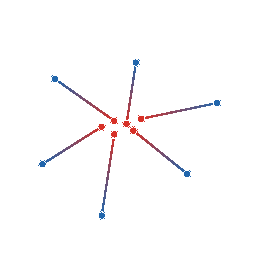
\includegraphics[width=.235\linewidth]{figures/sinkhorn-path-space-bridges/eps-0.pdf} &
\index{path space}% strictindex
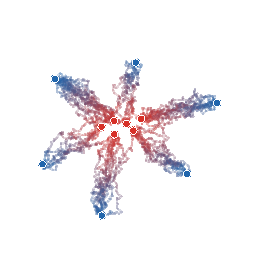
\includegraphics[width=.235\linewidth]{figures/sinkhorn-path-space-bridges/eps-0p035.pdf} &
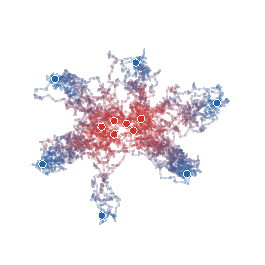
\includegraphics[width=.235\linewidth]{figures/sinkhorn-path-space-bridges/eps-0p10.pdf} &
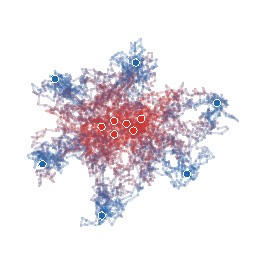
\includegraphics[width=.235\linewidth]{figures/sinkhorn-path-space-bridges/eps-0p28.pdf} \\[-.1em]
\small $\epsilon=0$ &
\small $\epsilon=0.035$ &
\small $\epsilon=0.10$ &
\small $\epsilon=0.28$
\end{tabular}
\caption{\emph{Schematic endpoint couplings lifted to Brownian bridges.} Each panel transports six equally weighted red atoms concentrated near the center to six blue atoms distributed around them. For the displayed value of $\epsilon$, the endpoint coupling is either the exact quadratic OT plan ($\epsilon=0$) or the entropic Sinkhorn plan ($\epsilon>0$). A total of 60 paths is sampled by a multinomial allocation with probabilities $\pi_{i,j}$, and each selected pair $(x_i,y_j)$ is filled by a Brownian bridge with covariance proportional to $\epsilon t(1-t)$. Colors encode time from red to blue; probabilistically, the discrete picture corresponds to a reciprocal mixture of endpoint-conditioned bridges.}
\index{endpoint coupling}% strictindex
\index{bridge!Brownian}% strictindex
\label{fig:sinkhorn-path-space-bridges}
\end{figure}

The deterministic and entropic path-space formulations thus differ in how each transported endpoint pair is filled: by a least-action path in the former and by a conditional reference bridge in the latter. We now return to deterministic transport and vary its instantaneous action to generate other dynamic geometries.

%%%%%%%%%%%%%%%%%%%%%%%%%%%%%%%%%%%%%%%%%%%%%%%%%%%%%%%%%%%%%%%%%%%%%%%%%%%

\section{Generalized Dynamic Wasserstein Distances}
\index{dynamic!formulation}% strictindex
\label{sec-bb-extensions}
\label{sec-generalized-dynamic-wasserstein-distances}

The quadratic Benamou--Brenier formula is only one instance of a broader fixed-mass dynamic language. The goal of this section is to construct a large family of geodesic-like geometries on spaces of probability measures by modifying the action minimized in the Benamou--Brenier formula. An arbitrary action first defines only a path value; metric properties require the symmetry, homogeneity and closure hypotheses isolated below. All descent constructions are postponed to Section~\ref{sec-generalized-dynamic-wasserstein-flows}, where the resulting distances are used to generate gradient-flow PDE models.
\index{Wasserstein!distance}% strictindex
\index{perspective function}% strictindex

\paragraph{Path actions.}
\index{path action}% strictindex
The common starting point is an instantaneous cost for moving a measure with a prescribed Eulerian velocity. Integrating this cost along continuity-equation curves produces the associated endpoint geometry.

In the mass-preserving Euclidean setting, the basic input is an instantaneous action $\mathbb A(\alpha,w)$, where \(\alpha\) is the current measure and \(w\) is an admissible velocity representative. Its endpoint geometry is defined dynamically.
\begin{defn}[Generalized dynamic action value]\label{def-generalized-dynamic-action-distance}
Let $\mathbb A$ be a nonnegative extended-valued action on measure--velocity pairs. Define
\begin{equation}\label{eq-generalized-action-length-distance}
	\mathsf E_{\mathbb A}(\alpha_0,\alpha_1)
	\eqdef
	\inf_{\alpha_t,v_t}
	\left\{
	\int_0^1 \mathbb A(\alpha_t,v_t)\,\d t
	:
	\partial_t\alpha_t+
	\diverg(\alpha_t v_t)=0,\
	\alpha_{t=0}=\alpha_0,\
		\alpha_{t=1}=\alpha_1
	\right\}.
\end{equation}
\end{defn}
Equivalently, one may quotient by velocity fields that induce the same first-order variation of the measure. The value~\eqref{eq-generalized-action-length-distance} need not be symmetric or separate measures, and its square root need not satisfy the triangle inequality. For an action that is $r$-homogeneous in velocity and satisfies the hypotheses of Proposition~\ref{prop-homogeneous-dynamic-action-distance}, the associated distance is instead the $r$-th root of this value. Some standard distances, such as \(\Wass_p\), are first written with a \(p\)-homogeneous action and then squared by taking a constant-speed parametrization; this normalization is made explicit below. Different choices of \(\mathbb A\) change the resulting geometry; Section~\ref{sec-generalized-dynamic-wasserstein-flows} later reuses these choices when dynamics are introduced.

\paragraph{Quadratic, or Riemannian, tangent actions.}
\index{local tangent action}% strictindex
\index{squared local action}% strictindex
\index{local action}% strictindex
\index{tangent action}% strictindex
\index{length space}% strictindex
\index{geodesic!distance}% strictindex
\index{quadratic!action}% strictindex
\index{Onsager operator}% strictindex
\index{Riemannian metric}% strictindex
\index{tangent norm}% strictindex
\index{quadratic!tangent norm}% strictindex
A particularly transparent case occurs when \(w\mapsto\mathbb A(\alpha,w)\) is quadratic. For simplicity, take admissible velocities in \(L^2(\alpha;\RR^d)\); in some applications this Hilbert space is replaced by a closed subspace encoding additional constraints. If the polarization of \(\mathbb A\) is represented by a positive self-adjoint operator
\(Q_\alpha:L^2(\alpha;\RR^d)\to L^2(\alpha;\RR^d)\),
\[
	\mathbb A(\alpha;w,z)
	=
	\left\langle Q_\alpha w,z\right\rangle_{L^2(\alpha)},
	\qquad
	\mathbb A(\alpha,w)=\left\langle Q_\alpha w,w\right\rangle_{L^2(\alpha)},
\]
	and if the quadratic form is nondegenerate after quotienting velocities that induce the same measure variation, then the associated quadratic path value is
\begin{equation}\label{eq-general-quadratic-tangent-action}
	\mathsf D_Q^2(\alpha_0,\alpha_1)
	=
	\mathsf E_{\mathbb A}(\alpha_0,\alpha_1)
	=
	\inf_{\substack{\partial_t\alpha_t+\diverg(\alpha_t v_t)=0\\
	\alpha_{t=0}=\alpha_0,\ \alpha_{t=1}=\alpha_1}}
	\int_0^1
	\left\langle Q_{\alpha_t}v_t,v_t\right\rangle_{L^2(\alpha_t)}
	\d t.
\end{equation}
When, in addition, the dynamic problem is sequentially closed and attains finite infima as in Proposition~\ref{prop-homogeneous-dynamic-action-distance}, $\mathsf D_Q$ is an extended distance. The usual $\Wass_2$ geometry corresponds to $Q_\alpha=\Id$ in this simplified notation. Thus \(Q_\alpha\) records how the chosen geometry deforms the Euclidean \(L^2(\alpha)\) tangent norm: no deformation for \(\Wass_2\), and a nontrivial tensor for generalized Riemannian geometries. In Section~\ref{sec-generalized-dynamic-wasserstein-flows}, the same tensor is reused as a preconditioner for metric descent.
\index{Hilbertian tangent norm}% strictindex
\index{Riemannian tensor}% strictindex
\index{Riemannian metric}% strictindex

\paragraph{Local velocity actions.}
\index{action density}% strictindex
\index{momentum variable}% strictindex
\index{momentum formulation}% strictindex
Many dynamic distances are local with respect to a reference measure $\lambda$. Write $\alpha=a\lambda$. A velocity action is specified by a pointwise integrand
\[
	A:[0,+\infty)\times\RR^d\to[0,+\infty],
	\qquad
	(a,w)\mapsto A(a,w),
\]
where $a\in\RR_+$ is a density value and $w\in\RR^d$ is a velocity value, and defines
\begin{equation}\label{eq-local-velocity-action}
	\mathbb A(\alpha,w)
	=
	\int A\left(\frac{\d\alpha}{\d\lambda}(x),w(x)\right)\d\lambda(x).
\end{equation}
For a fixed reference $\lambda$, this covers density-dependent mobilities and congestion constraints. If, in addition, $A$ is positively $1$-homogeneous in its first variable, $A(\eta a,w)=\eta A(a,w)$ for $\eta\geq0$, then the same formula is intrinsic: replacing $\lambda$ by another dominating measure gives the same value. The usual Benamou--Brenier action is the model case
\begin{equation}\label{eq-bb-velocity-action}
	A_2(a,w)=a\norm{w}^2,
	\qquad
	\mathbb A(\alpha,w)=\int\norm{w}^2\d\alpha.
\end{equation}
Here \(a=\d\alpha/\d\lambda\) is the density of transported mass and \(w\) is the Eulerian velocity. The factor \(a\) says that moving twice as much mass with the same velocity costs twice as much.

\paragraph{Homogeneous momentum actions.}\label{rem-generalized-bb}
\index{Benamou-Brenier@Benamou--Brenier}% strictindex
\index{Benamou-Brenier@Benamou--Brenier!distance}% strictindex
\index{convex!action density}% strictindex
The same action can be written in momentum variables, and this is the form in which convexity and metric properties are easiest to read. Set $\omega=\alpha w$, so that $\omega$ is a vector-valued measure. When the local description is written with the same reference $\lambda$, so that $\alpha=a\lambda$ and $\omega=m\lambda$, the pointwise momentum perspective is
\begin{equation}\label{eq-general-momentum-perspective}
	J_A(a,m)
	\eqdef
	\begin{cases}
	A(a,m/a), & a>0,\\
	0, & a=0\ \text{and}\ m=0,\\
	+\infty, & a=0\ \text{and}\ m\neq0,
	\end{cases}
\end{equation}
and the measure action relative to $\lambda$ is
\begin{equation}\label{eq-general-measure-momentum-action}
	\mathbb J_{A,\lambda}(\alpha,\omega)
	\eqdef
	\int
	J_A\!\left(
		\frac{\d\alpha}{\d\lambda},
		\frac{\d\omega}{\d\lambda}
	\right)\d\lambda,
\end{equation}
with value \(+\infty\) if \(\alpha\) or the total variation \(|\omega|\) is not absolutely continuous with respect to \(\lambda\). This zero-density convention is the lower-semicontinuous one for the superlinear actions used below; other growths use the corresponding recession extension. If $A$ is positively $1$-homogeneous in $a$, then $J_A$ is jointly $1$-homogeneous: $J_A(\eta a,\eta m)=\eta J_A(a,m)$. In that intrinsic case the value of \(\mathbb J_{A,\lambda}\) is independent of the dominating reference measure, and we write simply \(\mathbb J_A\). For $A_2(a,w)=a\norm{w}^2$, one recovers the quadratic perspective
\[
	J_2(a,m)=\frac{\norm{m}^2}{a},
\]
which is the integrand used in the convex Benamou--Brenier formulation~\eqref{eq:benamou-brenier-convex}. In this case \(\omega=\alpha w\); if \(\alpha=\rho\d x\) and \(\omega=m\d x\), then \(m=\rho w\), and \(J_2(\rho,m)=\rho\norm w^2\).
\index{perspective function}% strictindex
\index{quadratic!perspective}% strictindex

\begin{prop}[Concave mobilities give convex momentum actions]\label{prop-momentum-perspective-convexity}
\index{perspective function}% strictindex
\index{convex!action density}% strictindex
\index{momentum formulation}% strictindex
	Let \(I\subset[0,+\infty)\) be a convex interval, let \(\theta:I\to[0,+\infty)\) be concave, and let \(L:\RR^d\to[0,+\infty]\) be convex with \(L(0)=0\). Define, on the set where \(\theta(a)>0\),
	\begin{equation}\label{eq-concave-mobility-perspective}
		J_{\theta,L}(a,m)
		\eqdef
		\theta(a)L\!\left(\frac{m}{\theta(a)}\right),
		\qquad
		A_{\theta,L}(a,w)
		\eqdef
		J_{\theta,L}(a,aw)
		=
		\theta(a)L\!\left(\frac{aw}{\theta(a)}\right),
	\end{equation}
	and extend \(J_{\theta,L}\) to the boundary by lower semicontinuity. Then \(J_{\theta,L}\) is convex in \((a,m)\). In particular, this single construction contains
	\[
		A(a,w)=aL(w)
		\quad\text{by taking }\theta(a)=a,
	\]
	and the concave-mobility quadratic action
	\[
		A(a,w)=\frac{a^2\norm{w}^2}{\theta(a)}
		\quad\text{by taking }L(u)=\norm u^2.
	\]
\end{prop}

\begin{proof}
	The perspective \(P(s,m)=sL(m/s)\) of a convex function is convex on \(s>0\). Since \(L(0)=0\), it is also nonincreasing in the scalar \(s\) for fixed \(m\): if \(s_2\geq s_1>0\), then
	\[
		L(m/s_2)
		=
		L\big((s_1/s_2)(m/s_1)\big)
		\leq
		(s_1/s_2)L(m/s_1),
	\]
	hence \(P(s_2,m)\leq P(s_1,m)\). Let \(a_\zeta=(1-\zeta)a_0+\zeta a_1\) and \(m_\zeta=(1-\zeta)m_0+\zeta m_1\). By concavity of \(\theta\),
	\[
		\theta(a_\zeta)
		\geq
		(1-\zeta)\theta(a_0)+\zeta\theta(a_1).
	\]
	Using the monotonicity in \(s\), and then the convexity of \(P\), gives
	\[
		J_{\theta,L}(a_\zeta,m_\zeta)
		=
		P(\theta(a_\zeta),m_\zeta)
		\leq
		P((1-\zeta)\theta(a_0)+\zeta\theta(a_1),m_\zeta)
		\leq
		(1-\zeta)J_{\theta,L}(a_0,m_0)+\zeta J_{\theta,L}(a_1,m_1).
	\]
	The boundary cases follow by the chosen lower-semicontinuous extension.
	\end{proof}

\begin{rem}[Perspective transform gives convexity]\label{rem-perspective-transform-convexity-link}
\index{perspective transform}% strictindex
\index{convexity!perspective transform}% strictindex
	The convexity mechanism in Proposition~\ref{prop-momentum-perspective-convexity} is the same one used earlier for $\phi$-divergences. In both cases one starts from a convex function of a ratio and multiplies by the denominator: the density-ratio perspective \(v\phi(u/v)\) proves the joint convexity and lower-semicontinuity of \(\Divergm_\phi\) in Proposition~\ref{prop-basic-phi-divergence-properties}, see \eqref{eq-phi-div} and \eqref{eq-discr-diverg}; the momentum perspective \(J_A(a,m)=A(a,m/a)\) in \eqref{eq-general-momentum-perspective} plays the same role for dynamic transport actions. The classical Benamou--Brenier relaxation uses the quadratic perspective \(J(a,m)=\norm{m}^2/a\) from \eqref{eq-quadratic-perspective}--\eqref{eq-measure-perspective-action}; concave mobilities use the modified perspective \eqref{eq-concave-mobility-perspective}; and unbalanced dynamic transport uses the three-variable analogue \(J_\kappa(a,m,r)\) in \eqref{eq-wfr-momentum-perspective}--\eqref{eq-wfr-measure-action}. Thus the same perspective transform is the hidden convexification behind density-ratio divergences, balanced dynamic OT, concave-mobility distances and Wasserstein--Fisher--Rao dynamics.
\end{rem}

The next proposition isolates the additional assumptions under which the momentum formulation generated by \(A\) defines a genuine path metric rather than only a variational principle.
\index{dynamic!formulation}% strictindex
\index{lower semicontinuous relaxation}% strictindex

\begin{prop}[Homogeneous dynamic actions define distances]\label{prop-homogeneous-dynamic-action-distance}
\index{dynamic!distance}% strictindex
\index{homogeneous action}% strictindex
\index{finite-action component}% strictindex
	Fix a reference measure \(\lambda\), omitted from the notation only in the intrinsic case where \(\mathbb J_{A,\lambda}\) does not depend on \(\lambda\). Assume that the momentum perspective \(J_A\) defined in~\eqref{eq-general-momentum-perspective} is lower semicontinuous, convex in \((a,m)\), even in \(m\), and satisfies \(J_A(a,0)=0\) on its effective density domain. Assume moreover that, for some \(r>1\),
	\[
			J_A(a,\xi m)=|\xi|^rJ_A(a,m)
			\qquad
			\text{for all admissible }a,\ \text{all }m,\ \text{and all }\xi\in\RR,
	\]
	and that, for each admissible $a$, \(J_A(a,m)=0\) if and only if \(m=0\). Equivalently, the evenness, homogeneity and nondegeneracy assumptions translate, away from zero density, into
	\[
		A(a,-w)=A(a,w),
		\qquad
		A(a,\xi w)=|\xi|^rA(a,w),
		\qquad
		A(a,w)=0 \Longleftrightarrow w=0
		\qquad (a>0\text{ admissible}).
	\]
	For a mass $M\geq0$, define the effective state space
	\[
		\mathcal S_{A,\lambda}^M
		\eqdef
		\left\{\alpha=a\lambda:\ \alpha(\mathcal X)=M,
		J_A(a(x),0)=0\ \lambda\text{-a.e.}\right\}.
	\]
	For endpoints in $\mathcal S_{A,\lambda}^M$, define
	\[
		\mathsf D_{A,\lambda}(\alpha_0,\alpha_1)
		\eqdef
		\inf_{\substack{\partial_t\alpha_t+\diverg\omega_t=0\\
		\alpha_{t=0}=\alpha_0,\ \alpha_{t=1}=\alpha_1}}
		\left(
		\int_0^1\mathbb J_{A,\lambda}(\alpha_t,\omega_t)\,\d t
		\right)^{1/r}.
	\]
	Assume finally that the relaxed dynamic problem is sequentially closed and attains its infimum whenever the value is finite. Then \(\mathsf D_{A,\lambda}\) is an extended distance on $\mathcal S_{A,\lambda}^M$, and a genuine distance on each finite-action component: it is symmetric, satisfies the triangle inequality, and \(\mathsf D_{A,\lambda}(\alpha_0,\alpha_1)=0\) only when \(\alpha_0=\alpha_1\). In the intrinsic case, the reference can be omitted and the same conclusion holds on the corresponding effective fixed-mass state space; we write \(\mathsf D_A\).
\end{prop}

\begin{proof}
	The constant curve \(\alpha_t=\alpha_0\), \(\omega_t=0\), gives \(\mathsf D_{A,\lambda}(\alpha_0,\alpha_0)=0\). Conversely, if \(\mathsf D_{A,\lambda}(\alpha_0,\alpha_1)=0\), attainment provides a relaxed zero-action minimizer, which satisfies
	\[
		\int_0^1 \mathbb J_{A,\lambda}(\alpha_t,\omega_t)\,\d t=0.
	\]
	Since \(\mathbb J_{A,\lambda}\geq0\), this implies \(\omega_t=0\) for a.e.\ \(t\). The continuity equation then gives \(\partial_t\alpha_t=0\) in the sense of distributions, so \(\alpha_0=\alpha_1\).

	Symmetry follows by time reversal. If \((\alpha_t,\omega_t)_{t\in[0,1]}\) connects \(\alpha_0\) to \(\alpha_1\), then
	\[
		\widetilde\alpha_t=\alpha_{1-t},
		\qquad
		\widetilde\omega_t=-\omega_{1-t}
	\]
	connects \(\alpha_1\) to \(\alpha_0\), satisfies the same continuity equation, and has the same action because \(J_A\) is even in \(m\).

	It remains to prove the triangle inequality. Let \((\alpha^1,\omega^1)\) connect \(\alpha_0\) to \(\alpha_1\) with action \(E_1\), and let \((\alpha^2,\omega^2)\) connect \(\alpha_1\) to \(\alpha_2\) with action \(E_2\). For \(\tau\in(0,1)\), concatenate the two curves after the time changes \(s=t/\tau\) and \(s=(t-\tau)/(1-\tau)\):
	\[
		(\alpha_t,\omega_t)=
		\begin{cases}
			\bigl(\alpha^1_{t/\tau},\,\tau^{-1}\omega^1_{t/\tau}\bigr), & 0\leq t\leq \tau,\\[.2em]
			\bigl(\alpha^2_{(t-\tau)/(1-\tau)},\,(1-\tau)^{-1}\omega^2_{(t-\tau)/(1-\tau)}\bigr), & \tau\leq t\leq1.
		\end{cases}
	\]
	The rescaled curve is admissible from \(\alpha_0\) to \(\alpha_2\). By \(r\)-homogeneity in the momentum variable, its action is
	\(\tau^{1-r}E_1+(1-\tau)^{1-r}E_2\).
	Writing \(X=E_1^{1/r}\) and \(Y=E_2^{1/r}\), the optimal allocation is \(\tau=X/(X+Y)\), with the evident limiting convention if \(X+Y=0\), and gives
	\[
		\inf_{\tau\in(0,1)}
		\left\{\tau^{1-r}E_1+(1-\tau)^{1-r}E_2\right\}
		=
		(X+Y)^r.
	\]
	Hence \(\mathsf D_{A,\lambda}(\alpha_0,\alpha_2)\leq E_1^{1/r}+E_2^{1/r}\). Taking \(E_1\) and \(E_2\) arbitrarily close to the two optimal action values yields
	\[
		\mathsf D_{A,\lambda}(\alpha_0,\alpha_2)
		\leq
		\mathsf D_{A,\lambda}(\alpha_0,\alpha_1)+\mathsf D_{A,\lambda}(\alpha_1,\alpha_2),
	\]
	with the usual extended-real convention when one of the distances is infinite.
\end{proof}

Without homogeneity or nondegeneracy, the same momentum action remains useful as a variational principle, but its \(r\)-th root need not define a distance.

\begin{example}[Wasserstein-\texorpdfstring{$p$}{p} action]
\index{Wasserstein!p-action@$p$-action}% strictindex
	The usual $\Wass_p$ distances correspond to changing only the homogeneity of the Benamou--Brenier action. The case $p=2$ is the original formula~\cite{benamou2000computational}; for $1<p<+\infty$, the same dynamic viewpoint gives the standard description of absolutely continuous curves in Wasserstein spaces~\cite{ambrosio2006gradient,Villani03,SantambrogioBook}. The specific objects to insert in the general framework above are
	\[
		A_p(a,w)=a\norm{w}^p,
		\qquad
		J_p(a,m)=
		\begin{cases}
			\norm{m}^p/a^{p-1}, & a>0,\\
			0, & (a,m)=(0,0),\\
			+\infty, & a=0,\ m\neq 0,
		\end{cases}
	\]
	With \(A=A_p\), Proposition~\ref{prop-homogeneous-dynamic-action-distance} gives the usual identity \(\mathsf D_{A_p}=\Wass_p\). The corresponding squared length-space normalization is
	\[
		\mathbb A_p(\alpha,w)
		=
		\left(\int\norm{w}^p\d\alpha\right)^{2/p}.
	\]
	This is the squared version of the \(p\)-homogeneous action: minimizing \(\int_0^1\mathbb A_p(\alpha_t,v_t)\d t\) gives \(\Wass_p^2\) after constant-speed reparametrization. Thus \(A_p,J_p\) denote the local \(p\)-homogeneous velocity and momentum densities, whereas \(\mathbb A_p\) denotes the squared tangent action used in the length formulation. The endpoint $p=1$ can be treated separately: the perspective becomes \(J_1(a,m)=\norm m\), and the dynamic problem collapses to Beckmann's formulation of $\Wass_1$~\cite{Beckmann52}.
\index{Wasserstein!distance}% strictindex
\index{Beckmann!formulation}% strictindex
\end{example}

\paragraph{Concave-mobility actions.}
\index{mobility!concave}% strictindex
\index{convex!action density}% strictindex
\index{mobility!convexity mechanism}% strictindex
\index{mobility}% strictindex
One can instead keep a quadratic momentum action and change the mobility. Dolbeault, Nazaret and Savar\'e introduced this construction as a class of generalized transport distances adapted to nonlinear diffusion~\cite{dolbeault2009new}. The defining objects are collected below.
\begin{defn}[Concave-mobility dynamic distance]\label{def-concave-mobility-distance}
Let \(I\subset[0,+\infty)\) be a closed convex interval and let \(\theta:I\to[0,+\infty)\) be continuous and concave, with $\theta>0$ on the relative interior of $I$. Define the closed momentum perspective
\[
	J_\theta(a,m)
	\eqdef
	\begin{cases}
		\norm{m}^2/\theta(a), & a\in I,\ \theta(a)>0,\\
		0, & a\in I,\ \theta(a)=0,\ m=0,\\
		+\infty, & \text{otherwise}.
	\end{cases}
\]
The corresponding velocity action is
\[
	A_\theta(a,w)=J_\theta(a,aw),
	\qquad
	A_\theta(a,w)=\frac{a^2\norm{w}^2}{\theta(a)}\quad\text{when }\theta(a)>0.
\]
For a fixed reference measure $\lambda$ and a mass $M\geq0$, set
\[
	\mathcal S_{\theta,\lambda}^M
	\eqdef
	\left\{\alpha=a\lambda:\alpha(\mathcal X)=M,\ a(x)\in I\ \lambda\text{-a.e.}\right\},
	\qquad
	\mathsf W_{\theta,\lambda}(\alpha_0,\alpha_1)
	\eqdef
	\mathsf D_{A_\theta,\lambda}(\alpha_0,\alpha_1).
\]
\end{defn}
The convexity of \(J_\theta\) is the special case \(L(u)=\norm u^2\) of Proposition~\ref{prop-momentum-perspective-convexity}. This is why concavity of the mobility, rather than convexity, is the structural condition that makes the continuity-equation formulation convex.

Fix now a reference measure \(\lambda\). If \(\alpha=a\lambda\), the induced squared tangent action is
\[
	\mathbb A_{\theta,\lambda}(\alpha,w)
	=
	\int A_\theta(a(x),w(x))\,\d\lambda(x)
	=
	\int \frac{a(x)^2}{\theta(a(x))}\norm{w(x)}^2\,\d\lambda(x),
\]
where the integrand uses the closed convention in Definition~\ref{def-concave-mobility-distance}; the action is $+\infty$ if $\alpha\not\ll\lambda$ or $a(x)\notin I$ on a set of positive $\lambda$-measure. Equivalently, on the set where \(\theta(a(x))>0\),
\[
	\mathbb A_{\theta,\lambda}(\alpha,w)
	=
	\int \frac{a(x)}{\theta(a(x))}\norm{w(x)}^2\,\d\alpha(x).
\]
Hence this is a local Riemannian case, in the sense of~\eqref{eq-general-quadratic-tangent-action}, whenever the multiplier \(a(x)/\theta(a(x))\) is finite and positive. The associated tensor is the multiplication operator
\begin{equation}\label{eq-concave-mobility-q-alpha}
	\big(Q_{\theta,\lambda,\alpha}w\big)(x)
	=
	\frac{a(x)}{\theta(a(x))}w(x),
	\qquad
	\alpha=a\lambda,
\end{equation}
defined \(\alpha\)-a.e.\ on the set where \(\theta(a)>0\). Except for linear mobilities \(\theta(a)=ca\), and in particular the normalized case \(\theta(a)=a\) which recovers \(\Wass_2\), the pointwise velocity action \(A_\theta(a,w)\) is not positively \(1\)-homogeneous in the density variable \(a\). Consequently the construction is not intrinsic under a change of \(\lambda\): the resulting distance depends on the chosen reference measure and is finite only between endpoints that can be joined by a finite-action curve with \(\alpha_t\ll\lambda\).

The subscript \(\lambda\) recalls that the action is measured through the density \(a=\d\alpha/\d\lambda\).
	Equivalently, because this action is quadratic in the momentum, \(\mathsf W_{\theta,\lambda}^2\) is the path value~\eqref{eq-generalized-action-length-distance} with \(\mathbb A=\mathbb A_{\theta,\lambda}\).

\begin{prop}[Concave-mobility dynamic distances]\label{prop-concave-mobility-distance}
\index{mobility!concave}% strictindex
\index{dynamic!distance}% strictindex
	For a fixed reference measure \(\lambda\), and under the standard compactness hypotheses ensuring existence of relaxed minimizers~\cite{dolbeault2009new}, \(\mathsf W_{\theta,\lambda}=\mathsf D_{A_\theta,\lambda}\) is an extended distance on $\mathcal S_{\theta,\lambda}^M$ and a genuine metric on each finite-action component.
\end{prop}

\begin{proof}
	Proposition~\ref{prop-momentum-perspective-convexity}, applied with \(L(u)=\norm u^2\), gives convexity on the positive-mobility region. Continuity of $\theta$, the explicit zero-mobility convention, and the barrier outside the closed interval $I$ give its lower-semicontinuous extension $J_\theta$. It is even in \(m\), satisfies \(J_\theta(a,0)=0\) on $I$, and obeys
	\(J_\theta(a,\xi m)=|\xi|^2J_\theta(a,m)\).
	Moreover \(J_\theta(a,m)=0\) if and only if \(m=0\), with the boundary convention used in its definition. For the fixed reference \(\lambda\), the hypotheses of Proposition~\ref{prop-homogeneous-dynamic-action-distance} therefore hold with \(r=2\); the existence assumption is supplied by the compactness hypothesis in the statement. That proposition gives symmetry, separation and the triangle inequality for \(\mathsf D_{A_\theta,\lambda}\), hence for \(\mathsf W_{\theta,\lambda}\).
\end{proof}

The choice $\theta(a)=a$ recovers $\Wass_2$. Other choices encode different geometry: $\theta(a)=a^\gamma$ with $0<\gamma\leq1$ changes the cost of moving dilute mass, while $\theta(a)=a(1-a/M)$ on $[0,M]$ models a volume-filling or exclusion effect, since mobility vanishes both at vacuum and at the maximal density. The distance is comparable with $\Wass_2$ on classes where $\theta(a)$ is bounded above and below by positive multiples of $a$; otherwise zero-mobility barriers can make some pairs infinitely far apart. Its use as a geometry for nonlinear diffusion is discussed in Section~\ref{sec-generalized-dynamic-wasserstein-flows}.
\index{Benamou-Brenier@Benamou--Brenier}% strictindex

\paragraph{Dynamic spectral Wasserstein distances.}
\index{spectral Wasserstein!dynamic distance}% strictindex
\index{matrix!perspective}% strictindex
\index{spectral Wasserstein!distance}% strictindex
\index{spectral!tangent action}% strictindex
\index{velocity covariance}% strictindex
The static spectral distances of Section~\ref{sec-spectral-subspace-wasserstein} penalize a coupling through the covariance of its displacement. A dynamic version keeps the continuity equation but replaces the pointwise kinetic energy by a gauge of the whole velocity covariance. The resulting action is nonlocal in space: velocity directions are charged globally through their covariance, rather than independently at each point.

The spectral geometry charges the covariance of the velocity field through a monotone gauge. The corresponding action and length distance are defined together.
\begin{defn}[Dynamic spectral Wasserstein distance]\label{def-dynamic-spectral-wasserstein}
Let $\gamma$ be a monotone spectral gauge on $\mathbb S_+^d$. Define
\index{monotone!spectral gauge}% strictindex
\begin{equation}\label{eq-spectral-tangent-action}
	\mathbb A_\gamma(\alpha,v)
	\eqdef
	\gamma\!\left(\int v(x)v(x)^\top\d\alpha(x)\right).
\end{equation}
\eqllead{The associated distance is}{eq-dynamic-spectral-wasserstein}{
	\mathsf W_{\gamma,\mathrm{dyn}}^2(\alpha_0,\alpha_1)
	\eqdef
	\mathsf E_{\mathbb A_\gamma}(\alpha_0,\alpha_1).
}
\end{defn}
The trace gauge gives the usual Wasserstein tangent action, while the operator gauge $\gamma(M)=\lambda_{\max}(M)$ charges only the largest directional velocity variance.
In density--momentum variables, this corresponds to the measure action
\[
	\mathbb J_\gamma(\alpha,\omega)
	=
	\gamma\!\left(\int
	\left(\frac{\d\omega}{\d\alpha}\right)
	\left(\frac{\d\omega}{\d\alpha}\right)^\top
	\d\alpha\right),
\]
or, when \(\alpha=\rho\,\d x\) and \(\omega=m\,\d x\),
\[
	\mathbb J_\gamma(\rho,m)
	=
	\gamma\!\left(\int \frac{m(x)m(x)^\top}{\rho(x)}\,\d x\right).
\]
This functional is convex in the density--momentum fields \((\rho,m)\) by the matrix perspective, together with the monotonicity and convexity of \(\gamma\). It is nevertheless not, in general, obtained by integrating a pointwise action density, because the covariance is computed globally before applying \(\gamma\). Among spectral gauges, the linear ones are exactly the scaled traces $\gamma(M)=c\tr(M)$ with $c>0$. In that case the velocity and momentum densities are
\[
	A_{\mathrm{lin}}(a,w)=ca\norm w^2,
	\qquad
	J_{\mathrm{lin}}(a,m)=c\frac{\norm{m}^2}{a},
\]
and $c=1$ recovers the usual Benamou--Brenier action. A functional $M\mapsto\tr(GM)$ with nonscalar $G\succeq0$ is Loewner-monotone but not orthogonally invariant, hence is anisotropic rather than spectral.

The following result, in the form used for normalized spectral flows in~\cite{peyre2026muon}, shows that this dynamic construction is not merely infinitesimal: it exactly recovers the static displacement-covariance formulation.

\begin{prop}[Static/dynamic equality for spectral Wasserstein]\label{prop-static-dynamic-spectral-wasserstein}
	\index{static-dynamic equivalence}% strictindex
	\index{spectral Wasserstein!distance}% strictindex
	Let $\gamma$ be a monotone spectral gauge and let $\alpha_0,\alpha_1\in\Pp_2(\RR^d)$. Then
	\[
		\mathsf W_{\gamma,\mathrm{dyn}}^2(\alpha_0,\alpha_1)
		=
		\Wass_\gamma^2(\alpha_0,\alpha_1).
	\]
	The common value defines a distance on $\Pp_2(\RR^d)$; the triangle inequality is established by the robust representation in Proposition~\ref{prop-spectral-wasserstein-robust}.
\end{prop}

\begin{proof}
	We first prove $\mathsf W_{\gamma,\mathrm{dyn}}^2\leq\Wass_\gamma^2$. Let $\pi\in\Couplings(\alpha_0,\alpha_1)$ and let $(X,Y)\sim\pi$. Set $Z_t=(1-t)X+tY$ and $\alpha_t=(Z_t)_\sharp\pi$. Define the Eulerian velocity as the conditional mean
	\(v_t(z)\eqdef \EE[Y-X\mid Z_t=z]\).
	Then $(\alpha_t,v_t)$ solves the continuity equation. If
	\[
		M_\pi\eqdef\int(x-y)(x-y)^\top\d\pi(x,y),
		\qquad
		C_t\eqdef\int v_t(z)v_t(z)^\top\d\alpha_t(z),
	\]
	conditional Jensen gives \(C_t\preceq M_\pi\). Indeed, for every direction \(u\in\RR^d\),
	\[
		u^\top C_tu
		=
		\EE\!\left[\EE[\dotp{u}{Y-X}\mid Z_t]^2\right]
		\leq
		\EE[(\dotp{u}{Y-X})^2]
		=
		u^\top M_\pi u.
	\]
	By the Loewner monotonicity of $\gamma$,
	\(\int_0^1\gamma(C_t)\d t \leq \gamma(M_\pi)\).
	Taking the infimum over $\pi$ gives the first inequality.
	\index{Loewner order}% strictindex
	\index{Jensen inequality}% strictindex

	Conversely, let $(\alpha_t,v_t)$ be an admissible finite-action competitor. Since $\gamma$ is a finite positive gauge on the finite-dimensional cone $\mathbb S_+^d$, it is equivalent to the trace on this cone; hence finite spectral action implies the usual finite kinetic energy needed for the superposition principle. Thus there exists a probability law $\eta$ on absolutely continuous paths $\omega_\cdot$ such that $(e_t)_\sharp\eta=\alpha_t$ and $\dot\omega_t=v_t(\omega_t)$ for a.e.\ \(t\). Let $\pi=(e_0,e_1)_\sharp\eta$ be the induced endpoint coupling. With \(C_t=\int v_tv_t^\top\d\alpha_t\), Jensen's inequality along each path gives
	\[
		(\omega_1-\omega_0)(\omega_1-\omega_0)^\top
		=
		\left(\int_0^1\dot\omega_t\d t\right)
		\left(\int_0^1\dot\omega_t\d t\right)^\top
		\preceq
		\int_0^1\dot\omega_t\dot\omega_t^\top\d t.
	\]
	After integration over $\eta$,
	\(M_\pi\preceq \int_0^1 C_t\d t\).
	Monotonicity of $\gamma$, followed by convexity, yields
	\[
		\gamma(M_\pi)
		\leq
		\gamma\!\left(\int_0^1 C_t\d t\right)
		\leq
		\int_0^1\gamma(C_t)\d t.
	\]
	Since $\pi$ is admissible for the static problem, $\Wass_\gamma^2(\alpha_0,\alpha_1)$ is bounded by the action of the dynamic competitor. Taking the infimum over all competitors gives the reverse inequality.
	\index{superposition principle}% strictindex
	\index{path measure}% strictindex

	The crucial assumption is the monotonicity of $\gamma$: both parts of the proof produce Loewner-order comparisons between covariance matrices, and these comparisons imply inequalities between actions only for monotone gauges.
\end{proof}

The use of this geometry for normalized flows, including the operator-gauge connection with Muon-type normalization, is developed in Section~\ref{sec-normalized-spectral-wasserstein-dynamics}.
\index{operator gauge}% strictindex
\index{Muon algorithm}% strictindex

\paragraph{Kernelized Benamou--Brenier distances.}\label{sec-kernelized-bb-distance}
\index{kernelized transport distance}% strictindex
\index{RKHS!velocity}% strictindex
\index{Stein geometry}% strictindex
\index{Benamou-Brenier@Benamou--Brenier!kernelized}% strictindex
\index{Stein variational gradient descent}% strictindex
\index{RKHS!vector field}% strictindex
A different way to deform the Benamou--Brenier geometry is to keep the local continuity equation but to measure velocities in a reproducing-kernel Hilbert space rather than in $L^2(\alpha)$. This construction is motivated by Stein variational gradient descent, studied later in Section~\ref{sec-svgd-generative-flow}: the kernel makes the velocity field computable from particles, while its regularity is inherited from that of the kernel. The price is a much more restrictive transport geometry.

The kernelized distance uses a vector-valued RKHS as its restricted velocity class.
\begin{defn}[Kernelized Benamou--Brenier distance]\label{def-kernelized-bb-distance}
Let $k$ be a Borel measurable positive definite kernel on $\RR^d$ with scalar RKHS $\RKHS_k$. Set
\[
	\RKHS_k^d\eqdef \RKHS_k\times\cdots\times\RKHS_k,
	\qquad
	\norm{v}_{\RKHS_k^d}^2
	\eqdef
	\sum_{\ell=1}^d\norm{v_\ell}_{\RKHS_k}^2.
\]
\begin{equation}\label{eq-kernelized-bb-distance}
	\mathbb A_k(\alpha,v)
	\eqdef
	\norm{v}_{\RKHS_k^d}^2,
	\qquad
	\mathcal W_k^2(\alpha_0,\alpha_1)
	\eqdef
	\mathsf E_{\mathbb A_k}(\alpha_0,\alpha_1),
\end{equation}
where the infimum is restricted to strongly measurable $v\in L^2([0,1];\RKHS_k^d)$ satisfying the continuity equation.
\end{defn}
This is the vector-valued analogue of the scalar RKHS norm used for MMDs in Section~\ref{sec-rkhs-mmd}. Formula~\eqref{eq-generalized-action-length-distance} is restricted to velocities \(v_t\in\RKHS_k^d\). The action is independent of \(\alpha\); the measure enters only through the continuity equation. This type of Stein geometry was introduced in the analysis of SVGD by Liu and Wang~\cite{LiuWang2016SVGD,Liu2017SVGDGradientFlow} and later developed geometrically in~\cite{DuncanNueskenSzpruch2019SVGDGeometry,NueskenRenger2021SVGDAsymptotics}. The important caveat is that the admissible tangent space is the restricted RKHS class, not the whole Wasserstein tangent space; its regularity is determined by the assumptions on $k$.

\begin{prop}[Kernelized dynamic distance]\label{prop-kernelized-bb-distance}
\index{kernelized transport distance}% strictindex
\index{finite-action component}% strictindex
	Assume that the kernel has uniformly bounded diagonal,
	\[
		\kappa_k^2\eqdef\sup_{x\in\RR^d}k(x,x)<+\infty.
	\]
	Then the quantity \(\mathcal W_k\) defined by~\eqref{eq-kernelized-bb-distance} is an extended distance on probability measures. More precisely, it is symmetric, satisfies the triangle inequality, and \(\mathcal W_k(\alpha_0,\alpha_1)=0\) implies \(\alpha_0=\alpha_1\). It can take the value \(+\infty\) between different finite-action components.
\end{prop}

\begin{proof}
	The Borel assumption makes every RKHS function measurable: kernel sections are Borel, their finite linear span is Borel, and the bounded evaluation estimate below turns RKHS-norm convergence into uniform convergence. The constant curve gives zero self-distance. To prove separation without assuming existence of a minimizing curve, use the RKHS evaluation bound
	\(\norm{v(x)}\leq \kappa_k\norm{v}_{\RKHS_k^d}\).
	For every $\varphi\in C_c^1(\RR^d)$ and every admissible curve of action $E$, the weak continuity equation and Cauchy--Schwarz give
	\[
	\begin{aligned}
		\left|\int\varphi\,\d(\alpha_1-\alpha_0)\right|
		&\leq
		\int_0^1\!\int\norm{\nabla\varphi(x)}\,\norm{v_t(x)}\,\d\alpha_t(x)\d t\\
		&\leq
		\kappa_k\norm{\nabla\varphi}_\infty
		\left(\int_0^1\norm{v_t}_{\RKHS_k^d}^2\d t\right)^{1/2}
		=
		\kappa_k\norm{\nabla\varphi}_\infty\sqrt E.
	\end{aligned}
	\]
	Taking the infimum over admissible curves shows that $\mathcal W_k(\alpha_0,\alpha_1)=0$ forces equality of the integrals of every compactly supported smooth test function, hence $\alpha_0=\alpha_1$.

	Symmetry follows by time reversal and by replacing \(v_t\) with \(-v_{1-t}\). For the triangle inequality, concatenate an almost optimal curve from \(\alpha_0\) to \(\alpha_1\) of action \(E_1\) with one from \(\alpha_1\) to \(\alpha_2\) of action \(E_2\). Compressing the first curve into a time interval of length \(\tau\) multiplies its action by \(1/\tau\), and compressing the second into length \(1-\tau\) multiplies its action by \(1/(1-\tau)\). Optimizing over \(\tau\in(0,1)\) gives \((\sqrt{E_1}+\sqrt{E_2})^2\), and taking infima yields the triangle inequality.
\end{proof}

\index{finite-action component}% strictindex
\index{particle splitting}% strictindex
One should read \(\mathcal W_k\) as an extended distance on finite-action components, not as a replacement for $\Wass_2$ on all of $\Pp_2(\RR^d)$. A useful sufficient condition for finiteness is that the endpoints lie on the same RKHS-flow orbit: if there exists \(v\in L^2([0,1];\RKHS_k^d)\) whose flow map \(\Phi_t\) solves \(\dot\Phi_t=v_t\circ\Phi_t\) and satisfies \(\alpha_1=(\Phi_1)_\sharp\alpha_0\), then \(\mathcal W_k^2(\alpha_0,\alpha_1)\leq\int_0^1\norm{v_t}_{\RKHS_k^d}^2\d t\). For a concrete particle-level criterion, assume that $k$ is continuous and strictly positive definite and that $t\mapsto x_i(t)$ are pairwise-distinct absolutely continuous paths on $[0,1]$ with velocities $\dot x_i\in L^2(0,1)$. The Gram matrix $K_t=(k(x_i(t),x_j(t)))_{i,j}$ then varies continuously and is uniformly positive definite on the compact time interval. The minimum-norm RKHS interpolant with values $v_t(x_i(t))=\dot x_i(t)$ consequently has square-integrable norm, and discrete measures with the corresponding fixed weights lie at finite distance. Smooth or Lipschitz interpolating fields require the corresponding differentiability and RKHS embedding properties of $k$; strict positive definiteness alone does not provide such regularity.

The same condition also explains the limitation. If $k$ is smooth enough that $\RKHS_k^d$ embeds into Lipschitz vector fields, finite-action curves are induced by flows of regular maps. Atomic measures therefore remain atomic with the same number of atoms along such curves, so a Dirac mass cannot be transported at finite kernelized action to a measure with a density. This lack of splitting is precisely what makes the geometry useful for deterministic particle methods, and also what makes it a nontrivial extended object rather than a full probability metric.
\index{atomic measure}% strictindex
\index{regular vector field}% strictindex

\section{Nonlocal Wasserstein Distances}\label{sec-nonlocal-wasserstein-distances}
\index{nonlocal!action}% strictindex
\index{pair-space action}% strictindex
\index{nonlocal Wasserstein!distance}% strictindex
\index{jump process}% strictindex
\index{jump kernel}% strictindex
\index{reversible jump kernel}% strictindex
The local dynamic distances above transport mass through a vector field on the base space and a classical continuity equation. Nonlocal geometries use a different tangent model: the elementary motion is an exchange across an edge or a jump from \(x\) to \(y\). The common data are a reversible kernel \(K\), a symmetric edge or jump measure \(\mathsf J\), a pairwise increment \(\bar\nabla\), and a pair-space action \(\mathbb A_K\). The tangent variable is therefore attached to pairs of points, not to a single point \(x\), so these constructions are not simply obtained by choosing another pointwise local cost \(A(a,w)\).

There are two complementary versions. On a finite state space, the goal is to put a Wasserstein-like geometry on the probability simplex so that the entropy gradient flow is exactly a prescribed reversible Markov chain~\cite{Maas2011,MielkeCVPDE,ChowHuangLiZhou2012}. On a continuum space, the same edge calculus becomes a jump calculus over \(\mathcal X\times\mathcal X\), which models nonlocal motion, heavy-tailed jumps, and fractional-type diffusion; this is the construction of Erbar~\cite{Erbar2012JumpEntropy}, building on nonlinear mobilities~\cite{dolbeault2009new}, with subsequent metric and asymptotic refinements~\cite{SlepcevWarren2022NonlocalWasserstein}.

In both settings the canonical mobility for entropy is the logarithmic mean.
\begin{defn}[Logarithmic mean]\label{def-logarithmic-mean}
\begin{equation}\label{eq-logarithmic-mean}
\theta(a,b)\eqdef
\begin{cases}
\displaystyle\frac{a-b}{\log a-\log b}, & a,b>0\text{ and }a\neq b,\\[.4em]
a, & a=b,\\
0, & ab=0,
\end{cases}
\end{equation}
for $a,b\geq0$.
\end{defn}
For $a,b>0$, it satisfies \(\theta(a,b)(\log a-\log b)=a-b\); at vacuum, this relation is understood only as a limiting identity. This edge-wise chain rule identifies entropy-driven flows with the underlying reversible Markov or jump dynamics.
\index{logarithmic mean}% strictindex

\paragraph{Continuum jump kernels.}
\index{pair space}% strictindex
\index{mobility!nonlocal}% strictindex
The continuum version replaces graph edges by a symmetric measure on pairs. Weak compactness forces one to formulate the geometry for arbitrary measures and pair-flux measures; the more intuitive density--velocity formula is then an absolutely continuous specialization.

Let $(\mathcal X,d)$ be a Polish metric space, let $\mathfrak m$ be a Radon reference measure, and let $K(x,\cdot)$ be a nonnegative Borel kernel, possibly of infinite total mass. Assume that the pair measures introduced below are locally finite on the off-diagonal pair space $\mathcal G\eqdef\{(x,y)\in\mathcal X^2:x\neq y\}$ for the states under consideration. This is automatic under the Euclidean kernel assumptions used in Proposition~\ref{prop-nonlocal-distance-properties}. Define the jump measure $\mathsf J$ by
\begin{equation}\label{eq-nonlocal-jump-measure}
	\int_{\mathcal G}\Phi(x,y)\,\mathsf J(\d x,\d y)
	\eqdef
	\int_{\mathcal X}\left(\int_{\mathcal X\setminus\{x\}}\Phi(x,y)K(x,\d y)\right)\mathfrak m(\d x).
\end{equation}
Reversibility means that $\mathsf J$ is invariant under $(x,y)\mapsto(y,x)$. Write $\bar\nabla\varphi(x,y)\eqdef\varphi(y)-\varphi(x)$.

For a probability measure $\alpha$, introduce the two oriented edge measures
\begin{equation}\label{eq-nonlocal-oriented-edge-measures}
	\alpha^1(\d x,\d y)\eqdef K(x,\d y)\alpha(\d x),
	\qquad
	\alpha^2(\d x,\d y)\eqdef K(y,\d x)\alpha(\d y).
\end{equation}
If $\nu$ is a signed Radon measure on $\mathcal G$ and $\varsigma$ dominates $\alpha^1$, $\alpha^2$, and $|\nu|$, write $r_1=\d\alpha^1/\d\varsigma$, $r_2=\d\alpha^2/\d\varsigma$, and $q=\d\nu/\d\varsigma$. The logarithmic mean is positively $1$-homogeneous, so the closed perspective below is independent of the choice of $\varsigma$.

\begin{defn}[Continuum nonlocal Wasserstein distance]\label{def-continuum-nonlocal-wasserstein}
Define the relaxed pair action by
\begin{equation}\label{eq-nonlocal-relaxed-action}
	\mathbb A_K(\alpha,\nu)
	\eqdef
	\frac12\int_{\mathcal G}
	\begin{cases}
	\displaystyle\frac{|q|^2}{\theta(r_1,r_2)},&\theta(r_1,r_2)>0,\\[.35em]
	0,&\theta(r_1,r_2)=0,\ q=0,\\
	+\infty,&\theta(r_1,r_2)=0,\ q\neq0,
	\end{cases}
	\d\varsigma.
\end{equation}
An admissible pair consists of a narrowly continuous curve $(\alpha_t)_{t\in[0,1]}$ and a Borel family of antisymmetric signed flux measures $(\nu_t)_t$ such that
\[
	\int_0^1\!\int_{\mathcal G}(1\wedge d(x,y))\d|\nu_t|(x,y)\d t<+\infty
\]
and, for every test function $\varphi$ that is $C^1$ in time, bounded Lipschitz in space, and compactly supported in space when needed,
\begin{equation}\label{eq-nonlocal-continuity-weak}
	\int_0^1\!\int_{\mathcal X}\partial_t\varphi_t\d\alpha_t\d t
	+\frac12\int_0^1\!\int_{\mathcal G}\bar\nabla\varphi_t\d\nu_t\d t
	=
	\int_{\mathcal X}\varphi_1\d\alpha_1-
	\int_{\mathcal X}\varphi_0\d\alpha_0.
\end{equation}
The induced action distance is
\begin{equation}\label{eq-nonlocal-wasserstein-distance}
	\mathcal W_K^2(\alpha_0,\alpha_1)
	\eqdef
	\inf_{(\alpha_t,\nu_t)}\int_0^1\mathbb A_K(\alpha_t,\nu_t)\d t.
\end{equation}
\end{defn}

For the density specialization, let $\alpha=\rho\mathfrak m$ and
\begin{equation}\label{eq-nonlocal-density-flux}
	\nu(\d x,\d y)
	=
	v(x,y)\theta(\rho(x),\rho(y))\mathsf J(\d x,\d y),
\end{equation}
where $v$ is antisymmetric. Then $\alpha^1=\rho(x)\mathsf J$, $\alpha^2=\rho(y)\mathsf J$, and
\[
	\mathbb A_K(\alpha,\nu)
	=
	\frac12\int_{\mathcal G}|v(x,y)|^2\theta(\rho(x),\rho(y))\mathsf J(\d x,\d y).
\]
Thus the earlier density--velocity formula is recovered, but a minimizing relaxed curve need not remain absolutely continuous with respect to $\mathfrak m$.
\index{logarithmic mean}% strictindex
\index{nonlocal!continuity equation}% strictindex
\index{antisymmetric velocity}% strictindex

The definition above makes sense on a general Polish space, but its metric and compactness properties require assumptions on the jump kernel and the ambient topology. The following statement records the Euclidean theorem actually used here.
\begin{prop}[Metric properties of nonlocal transport]\label{prop-nonlocal-distance-properties}
\index{geodesic}% strictindex
\index{nonlocal Wasserstein!distance}% strictindex
	Let $\mathcal X=\RR^d$. Assume that $K$ and $\mathfrak m$ satisfy Assumption~1.1 of~\cite{Erbar2012JumpEntropy}: besides reversibility, the weighted kernels $(1\wedge\norm{x-y}^2)K(x,\d y)$ depend continuously on $x$ against bounded continuous tests and are uniformly integrable both near the diagonal and at infinity. Then $\mathcal W_K$ is an extended distance on $\Pp(\RR^d)$. Every finite-distance component is complete and geodesic, the infimum in~\eqref{eq-nonlocal-wasserstein-distance} is attained whenever it is finite, and a minimizer can be parametrized at constant speed.
\end{prop}
\begin{proof}
	The density in~\eqref{eq-nonlocal-relaxed-action} is a convex lower-semicontinuous perspective and is $1$-homogeneous in $(r_1,r_2,q)$. Hence the action is well defined independently of $\varsigma$. The logarithmic mean satisfies Assumption~2.1 of~\cite{Erbar2012JumpEntropy}. Proposition~3.4 there supplies compactness and closure of the measure--flux continuity equation, Proposition~4.3 supplies attainment and constant-speed parametrization, and Theorem~4.4 proves definiteness, completeness and the geodesic property. Symmetry follows by time reversal $(\alpha_t,\nu_t)\mapsto(\alpha_{1-t},-\nu_{1-t})$. Concatenating two curves and allocating time in proportion to the square roots of their actions gives the triangle inequality, exactly as in Proposition~\ref{prop-homogeneous-dynamic-action-distance}. The consequences for entropy dynamics and fractional PDE examples are developed in Section~\ref{sec-nonlocal-wasserstein-pdes}.
\end{proof}

For a fixed jump kernel, this geometry is genuinely nonlocal and does not coincide with ordinary $\Wass_2$. A local metric is recovered in a small-jump limit only if the kernel can transport through vacuum. More explicitly, set $\mathcal X=\RR^d$ and $\mathfrak m=\mathcal L^d$, and let $\eta(z)=\bar\eta(\norm{z})$ satisfy Assumptions~2.1--2.2 of~\cite{SlepcevWarren2022NonlocalWasserstein}, including radial monotonicity and the required tail and nondegeneracy bounds. Suppose that
\[
	M_2(\eta)\eqdef\int_{\RR^d}\norm{z}^2\eta(z)\,\d z\in(0,+\infty),
\]
and, for some $c,r_0>0$ and $s\in(0,2)$,
\begin{equation}\label{eq-small-jump-singular-lower-bound}
	\eta(z)\geq c\norm{z}^{-d-s}
		\qquad\text{whenever }0<\norm{z}<r_0.
\end{equation}
\eqllead{and define}{eq-small-jump-kernel-scaling}{
	K_\varepsilon(x,\d y)
	\eqdef
	\eta_\varepsilon(y-x)\,\d y,
	\qquad
	\eta_\varepsilon(z)
	\eqdef
	\varepsilon^{-d}\eta(z/\varepsilon).
}
Radiality implies symmetry and isotropy, and a change of variables gives
\begin{equation}\label{eq-small-jump-kernel-moments}
	\int\norm{y-x}^2K_\varepsilon(x,\d y)
	=
	\varepsilon^2M_2(\eta),
	\qquad
	\int (y-x)(y-x)^\top K_\varepsilon(x,\d y)
	=
	\varepsilon^2\frac{M_2(\eta)}{d}\Id.
\end{equation}
Equation~\eqref{eq-small-jump-kernel-moments} is the precise sense in which the second-moment jump scale is $\varepsilon$. To obtain a nontrivial local limit, one simultaneously accelerates the jump rate by $\varepsilon^{-2}$ and sets
\[
	\widehat K_\varepsilon
	\eqdef
	\frac{2d}{\varepsilon^2M_2(\eta)}K_\varepsilon,
	\qquad
	\int (y-x)(y-x)^\top\widehat K_\varepsilon(x,\d y)=2\Id.
\]
Multiplying a jump kernel by a constant $c>0$ divides the associated distance by $\sqrt c$. Theorem~1.3 of~\cite{SlepcevWarren2022NonlocalWasserstein} therefore gives, for endpoints supported in a fixed compact set,
\[
	\mathcal W_{\widehat K_\varepsilon}
	=
	\varepsilon\sqrt{\frac{M_2(\eta)}{2d}}\,
	\mathcal W_{K_\varepsilon}
	\underset{\varepsilon\to0}{\longrightarrow}
	\Wass_2.
\]
The singular lower bound~\eqref{eq-small-jump-singular-lower-bound} is essential for the logarithmic mean because $\theta(1,0)=0$. A smooth integrable profile, including the usual bounded compactly supported kernels, does not satisfy this theorem: in that regime a Dirac mass can be at infinite nonlocal distance from another compactly supported singular measure, although their $\Wass_2$ distance is finite~\cite[Proposition~1.1]{SlepcevWarren2022NonlocalWasserstein}.

There is a rigorous anisotropic extension for affine images of such kernels. If $B$ is invertible and
\[
	\eta_B(z)=|\det B|^{-1}\eta(B^{-1}z),
\]
define
\[
	K_{B,\varepsilon}(x,\d y)
	\eqdef
	\varepsilon^{-d}\eta_B\!\left(\frac{y-x}{\varepsilon}\right)\d y,
	\qquad
	\widehat K_{B,\varepsilon}
	\eqdef
	\frac{2d}{\varepsilon^2M_2(\eta)}K_{B,\varepsilon}.
\]
The change of variables $x=B\xi$, $y=B\zeta$, together with the $1$-homogeneity of the logarithmic mean, then gives
\[
	\mathcal W_{\widehat K_{B,\varepsilon}}(\alpha_0,\alpha_1)
	=
	\mathcal W_{\widehat K_\varepsilon}(B^{-1}_\sharp\alpha_0,B^{-1}_\sharp\alpha_1)
	\longrightarrow
	\Wass_2(B^{-1}_\sharp\alpha_0,B^{-1}_\sharp\alpha_1).
\]
The limiting accelerated covariance is $2BB^\top$, and the local velocity action is $\int v^\top(BB^\top)^{-1}v\,\d\alpha$. For a general anisotropic profile, the covariance gives this candidate action formally, but a convergence theorem additionally requires compactness, recovery sequences, tail control and vacuum connectivity; no broader claim is made here.
\index{small-jump limit}% strictindex

\paragraph{Discrete Wasserstein distances on Markov chains.}\label{sec-discrete-wasserstein-markov}
\index{finite-state transport}% strictindex
\index{logarithmic mean}% strictindex
\index{discrete!Wasserstein geometry}% strictindex
\index{Markov chain}% strictindex

The finite-state version keeps the same pair-space philosophy, but with a finite graph of admissible exchanges. It is not the naive Euclidean metric on the simplex. The key idea, introduced by Maas and independently developed in related forms by Mielke and by Chow--Huang--Li--Zhou, is to use the transition graph of a reversible Markov chain to define both the admissible directions and the mobility of the mass~\cite{Maas2011,MielkeCVPDE,ChowHuangLiZhou2012}. The resulting distance is the finite-dimensional counterpart of the Wasserstein geometry behind the heat equation, and it is also the geometric structure used in numerical work on discrete metric-measure spaces~\cite{ErbarDCDS,erbar2017computation}. Its entropy interpretation is stated later in Proposition~\ref{prop-discrete-markov-entropy-gradient}.
\index{Shannon entropy}% strictindex
\index{heat flow}% strictindex
\index{reversible Markov chain}% strictindex
\index{Maas distance}% strictindex

Let \(\mathcal X=\{1,\ldots,n\}\) and let \(K=(K_{i,j})\) denote the off-diagonal transition rates of an irreducible continuous-time Markov chain which is reversible with respect to a probability vector \(\pi\), so that \(\pi_iK_{i,j}=\pi_jK_{j,i}\) for \(i\neq j\). We write
\[
	\mathsf J_{i,j}\eqdef \pi_iK_{i,j}=\pi_jK_{j,i}
\]
for the symmetric edge measure, the finite counterpart of the jump measure used above. The transported object is a mass histogram
\[
\simplex_n\eqdef\left\{a\in\RR_+^n:\sum_i a_i=1\right\}.
\]
Relative densities only enter as auxiliary variables with respect to the invariant law:
\[
	\rho_i(a)\eqdef \frac{a_i}{\pi_i},
	\qquad a_i=\pi_i\rho_i(a).
\]
The logarithmic mean \(\theta\) defined in~\eqref{eq-logarithmic-mean} is the mobility selected so that the entropy calculus later recovers exactly the Markov evolution; see Proposition~\ref{prop-discrete-markov-entropy-gradient}. For positive $a,b$, the identity \(\theta(a,b)(\log a-\log b)=a-b\), extended to boundary states by approximation, converts entropy gradients into density differences along graph edges. For a potential \(\psi\in\RR^n\), set
\[
	\bar\nabla\psi(i,j)\eqdef\psi_j-\psi_i.
\]
The finite nonlocal divergence, tangent action, and distance are the discrete counterparts of Definition~\ref{def-continuum-nonlocal-wasserstein}.
\index{Onsager operator}% strictindex
\Needspace{26\baselineskip}
\begin{defn}[Discrete Markov-chain Wasserstein distance]\label{def-discrete-markov-wasserstein}
\index{Markov-chain Wasserstein geometry!distance}% strictindex
\begin{equation}
\label{eq-discrete-markov-onsager}
(\mathcal K_\rho\psi)_i
\eqdef
\sum_j K_{i,j}\theta(\rho_i,\rho_j)(\psi_i-\psi_j),
\qquad
(\mathcal L_a\psi)_i
\eqdef
\pi_i(\mathcal K_{\rho(a)}\psi)_i.
\end{equation}
Its associated tangent action is
\begin{equation}
\label{eq-discrete-markov-action}
\mathbb A_K(a,\psi)
\eqdef
\frac12\sum_{i,j}\mathsf J_{i,j}\theta(\rho_i(a),\rho_j(a))
(\bar\nabla\psi(i,j))^2.
\end{equation}
\begin{equation}
\label{eq-discrete-markov-distance}
\mathcal W_K^2(a_0,a_1)
\eqdef
\inf_{a_t,\psi_t}
\int_0^1\mathbb A_K(a_t,\psi_t)\,\d t,
\qquad
\dot a_t+\mathcal L_{a_t}\psi_t=0,
\end{equation}
with endpoint conditions \(a_{t=0}=a_0\) and \(a_{t=1}=a_1\).
\end{defn}
The tangent variable is the potential \(\psi\), or equivalently the induced edge flux, rather than an ambient Euclidean vector field. In edge-flux variables, flux is allowed only where \(K_{i,j}>0\), and its kinetic denominator is the logarithmic mean of the two relative endpoint densities.
\index{logarithmic mean}% strictindex
\index{Onsager operator}% strictindex
\index{edge flux}% strictindex

\index{simplex}% strictindex
The first nontrivial finite Markov geometries already show how the logarithmic mean bends the simplex. In both examples below, take the uniform random walk on the complete neighbor graph, i.e.\ every pair of distinct points is declared neighboring. Thus \(\pi_i=1/n\), and \(K_{i,j}=1/(n-1)\) for \(i\neq j\).
\index{random walk}% strictindex

\begin{example}[Two-point complete graph]
	On \(\simplex_2\), write \(a_0=(r,1-r)\) and \(a_1=(s,1-s)\). Since there is only one edge, the discrete dynamic problem reduces to the scalar Riemannian length
\begin{equation}
\label{eq-two-state-markov-distance}
\mathcal W_K(a_0,a_1)
=
\left|\int_s^r \frac{\d u}{\sqrt{\theta(u,1-u)}}\right|,
\qquad
0<r,s<1.
\end{equation}
	This formula is closed but not Euclidean: the logarithmic mean changes the cost of moving mass depending on the current split between the two points.
\end{example}
\index{logarithmic mean}% strictindex
\begin{example}[Three-point complete graph]
	Let $a_0,a_1\in\operatorname{int}(\simplex_3)$. The complete-neighbor graph is a triangle. For \(a\in\operatorname{int}(\simplex_3)\), set
\[
\Theta_{i,j}(a)\eqdef\frac12\theta(a_i,a_j),
\qquad 1\leq i<j\leq3.
\]
For a fixed \(a\), write \(\Theta_{i,j}=\Theta_{i,j}(a)\).
	For a tangent vector \(h\in\RR^3\) with \(h_1+h_2+h_3=0\), orient the edges as \(1\to2\), \(1\to3\), \(2\to3\). The squared norm induced by the discrete Wasserstein metric is
\index{discrete!Wasserstein geometry}% strictindex
\begin{equation}
\label{eq-three-state-markov-norm}
\|h\|_a^2
=
\min_{m_{1,2},m_{1,3},m_{2,3}}
\left\{
\frac{m_{1,2}^2}{\Theta_{1,2}}+
\frac{m_{1,3}^2}{\Theta_{1,3}}+
\frac{m_{2,3}^2}{\Theta_{2,3}}
\right\},
\end{equation}
subject to
\[
h_1+m_{1,2}+m_{1,3}=0,
\qquad
h_2-m_{1,2}+m_{2,3}=0,
\qquad
h_3-m_{1,3}-m_{2,3}=0.
\]
	Eliminating the three edge fluxes gives an explicit formula. With \(D=\Theta_{1,2}^{-1}+\Theta_{1,3}^{-1}+\Theta_{2,3}^{-1}\),
\[
m_{1,2}^*=\frac{h_2/\Theta_{2,3}-h_1/\Theta_{1,3}}{D},
\qquad
m_{1,3}^*=-h_1-m_{1,2}^*,
\qquad
m_{2,3}^*=m_{1,2}^*-h_2,
\]
and \(\|h\|_a^2\) is obtained by inserting these values in~\eqref{eq-three-state-markov-norm}. Therefore
\begin{equation}
\label{eq-three-state-markov-distance}
\mathcal W_K^2(a_0,a_1)
=
\inf_{a_t\in\operatorname{int}(\simplex_3)}
\int_0^1\|\dot a_t\|_{a_t}^2\,\d t,
\qquad
a_{t=0}=a_0,
\quad a_{t=1}=a_1.
\end{equation}
	Thus the three-state distance is an explicit two-dimensional Riemannian geodesic problem on the open triangle. The formula is simple enough to compute directly, but it already shows the main difference with Euclidean geometry on the simplex: the local metric depends nonlinearly on the current density through logarithmic edge mobilities.
\end{example}

Figure~\ref{fig:discrete-markov-simplex-distances} visualizes these small-dimensional geometries and compares them with the ordinary Wasserstein distance associated with the \(0/1\) ground metric, for which \(\Wass_2^2\) is one half of the total variation norm in~\eqref{eq-defn-tv}.
\index{total variation}% strictindex

\begin{figure}[H]
\centering
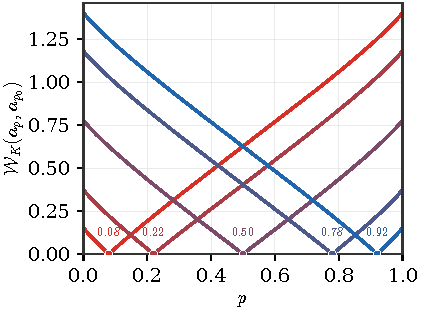
\includegraphics[width=.31\linewidth]{figures/discrete-markov-simplex-distances/sigma2-curves.pdf}
\hfill
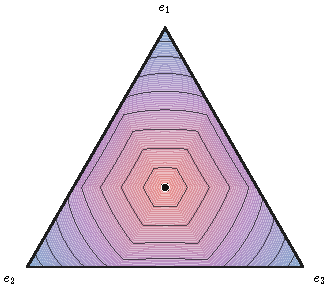
\includegraphics[width=.31\linewidth]{figures/discrete-markov-simplex-distances/sigma3-markov-levels.pdf}
\hfill
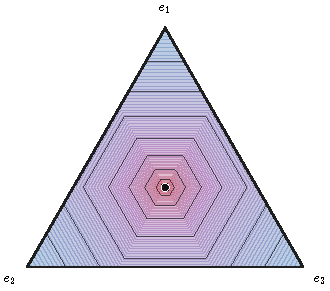
\includegraphics[width=.31\linewidth]{figures/discrete-markov-simplex-distances/sigma3-tv-levels.pdf}
\caption{\emph{Discrete Wasserstein distances on small Markov-chain simplices.} Left: the closed-form profiles \(r\mapsto \mathcal W_K(a_r,a_{r_0})\), with \(a_r=(r,1-r)\), for several anchors \(r_0\) on \(\simplex_2\). Middle: numerical level sets of \(\mathcal W_K(a,\bar a)\) on \(\simplex_3\), where \(\bar a=(1/3,1/3,1/3)\), computed from the local Riemannian norm induced by the complete-neighbor Markov chain. Right: the corresponding level sets for the ordinary \(\Wass_2\) distance with \(d(i,j)=1\) for \(i\neq j\), i.e.\ \(\Wass_2^2(a,\bar a)=\tfrac12\norm{a-\bar a}_{\mathrm{TV}}\).}
\label{fig:discrete-markov-simplex-distances}
\end{figure}

\section{Dynamic Unbalanced Wasserstein Distances}
\index{dynamic!unbalanced OT}% strictindex
\index{unbalanced!OT}% strictindex
\label{sec-unbalanced-ot}

Balanced dynamic distances keep the total mass fixed: their tangent vectors are transport velocities or fluxes satisfying a continuity equation. Unbalanced distances use a different tangent model. A tangent vector now has both a spatial component and a reaction component, so mass can move, disappear, and reappear. This section isolates this reaction--transport geometry before its use for gradient flows in Section~\ref{sec-dynamic-unbalanced-wfr-flows}.
\index{reaction-transport geometry}% strictindex
\index{unbalanced!tangent space}% strictindex

\paragraph{Balance equation and tangent variables.}
Unbalanced dynamic transport is obtained by allowing mass to be created and destroyed along the path. The continuity equation is replaced by a balance equation, and, at the density level, an admissible tangent direction is a pair \((m,s)\): the flux density \(m\) transports mass in space, while the source density \(s\) changes the amount of mass locally. This dynamic formulation underlies the Hellinger--Kantorovich and Wasserstein--Fisher--Rao metrics~\cite{LieroMielkeSavareShort,2017-chizat-focm}; its equivalence with static entropy-transport and cone formulations is developed in~\cite{LieroMielkeSavareLong,2015-chizat-unbalanced}. A representative quadratic balance equation is
\index{balance equation}% strictindex
\index{continuity equation}% strictindex
\index{growth term}% strictindex
\index{source term}% strictindex
	\[
		\partial_t\rho_t+\nabla\!\cdot m_t=s_t,
		\qquad
		\int_0^1\!\int
		\left(\frac{\norm{m_t}^2}{\rho_t}+\kappa^2\frac{s_t^2}{\rho_t}\right)\d x\,\d t,
	\]
	with the usual perspective convention: zero flux and zero source through zero density cost nothing, whereas nonzero flux or source through zero density has infinite cost. At the measure level these densities become the flux measure \(\omega_t=m_t\,\d x\) and the signed source measure \(\sigma_t=s_t\,\d x\).

\paragraph{Reaction--transport action.}
\index{reaction-transport action@reaction--transport action}% strictindex
The action attaches one price to displacement and another to local growth. Its velocity and momentum forms are collected in one definition.
\begin{defn}[Dynamic Wasserstein--Fisher--Rao distance]\label{def-dynamic-wfr-distance}
\index{Wasserstein-Fisher-Rao@Wasserstein--Fisher--Rao!dynamic distance}% strictindex
\eqllead{For $\kappa>0$, define}{eq-wfr-velocity-action}{
A_\kappa(a,w,g)\eqdef a\bigl(\norm{w}^2+\kappa^2g^2\bigr),
}
\eqllead{and}{eq-wfr-momentum-perspective}{
J_\kappa(a,m,r)\eqdef
\begin{cases}
(\norm{m}^2+\kappa^2r^2)/a,&a>0,\\
0,&(a,m,r)=(0,0,0),\\
+\infty,&a=0,\ (m,r)\neq(0,0).
\end{cases}
}
If $\lambda$ dominates $\alpha$, $|\omega|$, and $|\sigma|$, set
\begin{equation}\label{eq-wfr-measure-action}
\mathbb J_\kappa(\alpha,\omega,\sigma)
\eqdef
\int J_\kappa\!\left(\frac{\d\alpha}{\d\lambda},
\frac{\d\omega}{\d\lambda},\frac{\d\sigma}{\d\lambda}\right)\d\lambda.
\end{equation}
The induced dynamic Wasserstein--Fisher--Rao distance is
\begin{equation}\label{eq-dynamic-unbalanced-ot}
\WFR_\kappa^2(\alpha_0,\alpha_1)
\eqdef
\inf_{\substack{\partial_t\alpha_t+\nabla\cdot\omega_t=\sigma_t\\
\alpha_{t=0}=\alpha_0,\ \alpha_{t=1}=\alpha_1}}
\int_0^1\mathbb J_\kappa(\alpha_t,\omega_t,\sigma_t)\d t.
\end{equation}
\end{defn}
Here $w$ is velocity, $g$ is relative growth, $m=aw$ is flux, and $r=ag$ is source density. The parameter $\kappa$ fixes the relative cost of reaction and transport. Since \(J_\kappa\) is convex and positively one-homogeneous, the measure action is independent of \(\lambda\); finite action forces \(\omega,\sigma\ll\alpha\).
\index{balance equation}% strictindex
\index{Hellinger-Kantorovich@Hellinger--Kantorovich}% strictindex
\index{Wasserstein-Fisher-Rao@Wasserstein--Fisher--Rao}% strictindex

\paragraph{Static and dynamic viewpoints.}
The dynamic balance-equation formula is not a separate object from static unbalanced OT: it is the least-action representation of the same cone distance. To make the normalization explicit, define on the cone $\mathfrak C[\RR^d]$ the squared cost
\index{cone!metric}% strictindex
\begin{equation}\label{eq-wfr-scaled-cone-metric}
	\Delta_\kappa\big((x,r),(y,s)\big)^2
	\eqdef
	4\kappa^2
	\left[
		r^2+s^2-2rs
		\cos\!\left(
			\frac{\norm{x-y}}{2\kappa}\wedge\frac{\pi}{2}
		\right)
	\right].
\end{equation}
The radii encode masses through the weighted projection $\mathsf P_2$ defined in Section~\ref{sec-unbalanced}. Accordingly, set
\begin{equation}\label{eq-wfr-scaled-cone-value}
	\CW_\kappa(\alpha_0,\alpha_1)
	\eqdef
	\inf_{\substack{\gamma\in\Mm_+(\mathfrak C[\RR^d]^2)\\
	\mathsf P_2\gamma_1=\alpha_0,\ \mathsf P_2\gamma_2=\alpha_1}}
	\int
	\Delta_\kappa\big((x,r),(y,s)\big)^2
	\d\gamma(x,r,y,s).
\end{equation}
For $\kappa=1/2$, this is exactly the normalization of the Hellinger--Kantorovich cone cost used in Section~\ref{sec-unbalanced}. The next proposition identifies its general rescaling with the dynamic action above.

Thus Definition~\ref{def-dynamic-wfr-distance} gives both the reaction--transport action and the induced dynamic WFR metric.

\begin{prop}[Static/dynamic equivalence for unbalanced OT]\label{prop-static-dynamic-unbalanced}
\index{static-dynamic equivalence}% strictindex
\index{unbalanced!OT}% strictindex
	For nonnegative finite measures $\alpha_0,\alpha_1$ on $\RR^d$, the dynamic value~\eqref{eq-dynamic-unbalanced-ot} equals the static cone value~\eqref{eq-wfr-scaled-cone-value}. Hence $\WFR_\kappa=\CW_\kappa^{1/2}$ is the geodesic distance generated by the balance-equation least-action problem.
\end{prop}

\begin{proof}
	The cone construction turns variation of mass into radial motion and spatial transport into angular motion on $\mathfrak C[\RR^d]$. The normalization can be checked on a smooth cone path. If its base position is $x_t$, its cone radius is $r_t$, and the projected mass is $a_t=r_t^2$, then its relative growth rate is $g_t=\dot a_t/a_t=2\dot r_t/r_t$. The infinitesimal energy induced by~\eqref{eq-wfr-scaled-cone-metric} is therefore
	\[
		4\kappa^2\dot r_t^2+r_t^2\norm{\dot x_t}^2
		=
		a_t\left(\norm{\dot x_t}^2+\kappa^2g_t^2\right),
	\]
		which is precisely the velocity action~\eqref{eq-wfr-velocity-action}.

	The converse passage from an arbitrary Eulerian triple to a cone-valued dynamic plan is the substantive step. For $\kappa=1/2$, Theorems~4.3, 4.5 and 4.6 of~\cite{LieroMielkeSavareShort} provide respectively the dynamic-plan representation and the two action comparisons, and the proof of their Theorem~3.6 identifies the resulting distance with the cone metric. In their notation, the vector field is the chapter's velocity $w$, while the scalar field $\xi$ satisfies $g=4\xi$; hence their density $\norm w^2+4\xi^2$ is exactly $\norm w^2+\tfrac14g^2$. These theorems prove both inequalities for arbitrary finite measures, not only for smooth cone paths.

	For general $\kappa$, rescale the base metric by $(2\kappa)^{-1}$ and the cone distance by $2\kappa$. The same dynamic-plan theorem then gives the cone cost~\eqref{eq-wfr-scaled-cone-metric} and the action $\norm w^2+\kappa^2g^2$. This proves equality of the two infima. The corresponding complete-separable-space formulation and relaxation are developed in~\cite{LieroMielkeSavareLong}; related normalizations appear in~\cite{2017-chizat-focm,2015-chizat-unbalanced}.
	\index{cone!lifting}% strictindex
	\index{Benamou-Brenier@Benamou--Brenier}% strictindex
	\index{balance equation}% strictindex
	\index{lower semicontinuity}% strictindex
\end{proof}

\paragraph{Balanced versus unbalanced interpolations.}
\index{balanced interpolation}% strictindex
\index{unbalanced!interpolation}% strictindex
The distinction is visible already for one-dimensional mixtures with mismatched modal masses. Balanced transport must physically move the excess mass, whereas unbalanced transport can trade transport against reaction. Figure~\ref{fig:dynamic-unbalanced-geodesic} uses entropic balanced and KL-relaxed barycenters as a qualitative numerical surrogate; its unbalanced row illustrates the reaction--transport mechanism but is not asserted to be an exact $\WFR_\kappa$ geodesic.

\begin{figure}[H]
\centering
\setlength{\tabcolsep}{1pt}
\begin{tabular}{@{}rccccc@{}}
& \small $t=0$ & \small $t=.25$ & \small $t=.5$ & \small $t=.75$ & \small $t=1$ \\
\small balanced &
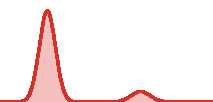
\includegraphics[width=.165\linewidth]{figures/dynamic-unbalanced-geodesic/balanced-t000.pdf} &
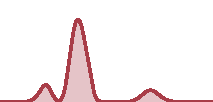
\includegraphics[width=.165\linewidth]{figures/dynamic-unbalanced-geodesic/balanced-t025.pdf} &
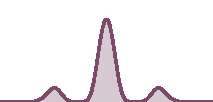
\includegraphics[width=.165\linewidth]{figures/dynamic-unbalanced-geodesic/balanced-t050.pdf} &
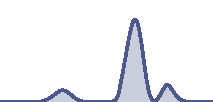
\includegraphics[width=.165\linewidth]{figures/dynamic-unbalanced-geodesic/balanced-t075.pdf} &
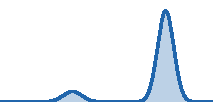
\includegraphics[width=.165\linewidth]{figures/dynamic-unbalanced-geodesic/balanced-t100.pdf} \\
\small unbalanced &
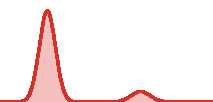
\includegraphics[width=.165\linewidth]{figures/dynamic-unbalanced-geodesic/unbalanced-t000.pdf} &
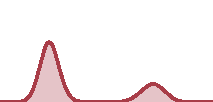
\includegraphics[width=.165\linewidth]{figures/dynamic-unbalanced-geodesic/unbalanced-t025.pdf} &
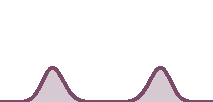
\includegraphics[width=.165\linewidth]{figures/dynamic-unbalanced-geodesic/unbalanced-t050.pdf} &
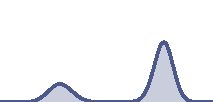
\includegraphics[width=.165\linewidth]{figures/dynamic-unbalanced-geodesic/unbalanced-t075.pdf} &
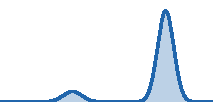
\includegraphics[width=.165\linewidth]{figures/dynamic-unbalanced-geodesic/unbalanced-t100.pdf}
\end{tabular}
\caption{\emph{Balanced and unbalanced Sinkhorn-barycenter interpolations between two one-dimensional Gaussian mixtures with swapped modal masses.} The balanced row conserves total mass, so excess mass from the dominant left mode must move along the line toward the dominant right target mode, producing transient mass in the middle. The unbalanced row uses KL-relaxed marginal constraints; mass can be attenuated near overrepresented modes and recreated near underrepresented modes, giving a reaction--transport interpolation closer to the Wasserstein--Fisher--Rao intuition.}
\index{Sinkhorn!barycenter}% strictindex
\index{unbalanced!barycenter}% strictindex
\label{fig:dynamic-unbalanced-geodesic}
\end{figure}

\section{Variational Mean Field Games}
\label{sec-variational-mean-field-games}
\index{mean field game}% strictindex
\index{variational!mean field game}% strictindex

Mean field games use a population law to summarize strategic interactions among a very large number of individually negligible agents. This section only considers the special \emph{potential} subclass in which the equilibrium system is the optimality condition of one convex planning problem. In that setting, the relation with dynamic OT is particularly transparent: one augments the Benamou--Brenier kinetic action by congestion and may replace a prescribed final measure by a terminal penalty. To state a closed problem without irrelevant issues at infinity, throughout this section $\Omega\subset\RR^d$ is a bounded connected Lipschitz domain, agents remain in $\overline\Omega$, and population flux has zero normal trace on $\partial\Omega$ in the sense of~\eqref{eq-continuity-endpoint-no-flux}.

\paragraph{From individual control to a population equilibrium.}
\index{Nash equilibrium}% strictindex
\index{population law}% strictindex
Mean field games were introduced by Lasry and Lions~\cite{LasryLions2007MeanFieldGames} and, in a parallel large-population stochastic-control framework, by Huang, Malham\'e and Caines~\cite{HuangMalhameCaines2006}. Given a candidate population density $(\rho_t)_{t\in[0,1]}$, a representative deterministic agent starting from $x\in\overline\Omega$ chooses an admissible path $\gamma:[0,1]\to\overline\Omega$ by minimizing
\begin{equation}\label{eq-mfg-individual-control}
	\inf_{\gamma(0)=x}
	\left\{
		\int_0^1
		\left(
			\frac12\norm{\dot\gamma(t)}^2
			+g\bigl(\rho_t(\gamma(t))\bigr)
		\right)\d t
		+\Psi(\gamma(1))
	\right\}.
\end{equation}
Here the kinetic term prices individual effort, $g(\rho)$ is the running cost created by the local population density, and the continuous function $\Psi:\overline\Omega\to\RR$ assigns a cost to the final state. A mean field Nash equilibrium requires consistency: when all agents use an optimal feedback for~\eqref{eq-mfg-individual-control}, the resulting law of their positions must be precisely $\alpha_t=\rho_t\,\d x$.

\paragraph{A Benamou--Brenier planning problem.}
\index{potential game}% strictindex
\index{congestion}% strictindex
The consistency condition is usually coupled to an individual Hamilton--Jacobi--Bellman equation. A global variational reduction is available when the local coupling is a first variation. Let $G:[0,+\infty)\to[0,+\infty]$ be proper, closed and convex with $G(0)=0$; in the differentiable case, assume
\begin{equation}\label{eq-mfg-congestion-primitive}
		g(r)=G'(r),
\end{equation}
while in general the coupling is selected from $g(r)\in\partial G(r)$. Starting from a probability density $\alpha_0=\rho_0\,\d x$ on $\Omega$, the associated potential MFG is the following planning problem.
\begin{defn}[Variational mean-field-game planning problem]\label{def-variational-mfg-planning}
\begin{equation}\label{eq-variational-mfg-velocity}
	\inf_{(\rho_t,v_t)}
	\left\{
		\int_0^1\!\int_{\Omega}
		\left(
			\frac12\rho_t(x)\norm{v_t(x)}^2+G(\rho_t(x))
		\right)\d x\,\d t
		+\int_{\Omega}\Psi(x)\rho_1(x)\d x
	\right\},
\end{equation}
\eqllead{subject to}{eq-variational-mfg-continuity}{
		\partial_t\rho_t+\diverg(\rho_t v_t)=0,
		\qquad
		\rho_{t=0}\,\d x=\alpha_0,
		\qquad
		(\rho_t v_t)\cdot n=0\ \text{on }\partial\Omega.
}
\end{defn}
Unlike in~\eqref{eq:benamou-brenier}, the final measure is not prescribed. The terminal potential $\Psi$ selects desirable final states softly, while the integral of $G(\rho_t)$ penalizes crowded intermediate configurations. It is important that the planner pays $G(\rho)$ rather than $\rho g(\rho)$: the marginal cost perceived by one infinitesimal agent is the first variation $G'(\rho)=g(\rho)$. For the usual congestion models, $g$ is nondecreasing, equivalently $G$ is convex; superlinear choices of $G$ increasingly penalize concentration.

This potential formulation and its deterministic and diffusive variants are developed by Benamou, Carlier and Santambrogio~\cite{BenamouCarlierSantambrogio2017}; first-order MFG systems with local couplings are analyzed, in particular, by Cardaliaguet and Graber~\cite{CardaliaguetGraber2015FirstOrderMFG}.

\paragraph{Convex momentum formulation.}
\index{momentum formulation}% strictindex
\index{mass flux}% strictindex
As in the Benamou--Brenier problem, the density--velocity integrand and the constraint in~\eqref{eq-variational-mfg-velocity}--\eqref{eq-variational-mfg-continuity} are not jointly convex. Set $\omega_t=\alpha_t v_t$, or $m_t=\rho_t v_t$ when densities exist. To obtain the weakly lower-semicontinuous congestion functional, write the Lebesgue decomposition $\alpha=\rho\,\d x+\alpha^s$ and set
\begin{equation}\label{eq-mfg-congestion-functional}
	\mathcal C_G(\alpha)
	\eqdef
	\int_\Omega G(\rho(x))\d x
		+G^\infty\alpha^s(\overline\Omega),
	\qquad
	G^\infty\eqdef\lim_{r\to+\infty}\frac{G(r)}r.
\end{equation}
For superlinear congestion, $G^\infty=+\infty$ and finite energy forces $\alpha\ll\d x$; the recession term is needed for closedness when $G$ has only linear growth.
Using the measure perspective action~\eqref{eq-measure-perspective-action}, the same problem becomes the generalized Benamou--Brenier formula
\begin{equation}\label{eq-variational-mfg-momentum}
	\inf_{(\alpha_t,\omega_t)}
	\left\{
		\int_0^1
		\left(
			\frac12\mathbb J(\alpha_t,\omega_t)
			+\mathcal C_G(\alpha_t)
		\right)\d t
		+\int_{\overline\Omega}\Psi\,\d\alpha_1
	\right\},
	\qquad
		\begin{gathered}
			\partial_t\alpha_t+\diverg\omega_t=0,
			\qquad \alpha_{t=0}=\alpha_0,\\
			\omega_t\cdot n=0\quad\text{on }\partial\Omega.
		\end{gathered}
	\end{equation}
Equivalently, in density--momentum variables, the running integrand is
\begin{equation}\label{eq-variational-mfg-density-momentum}
	\frac12J(\rho_t,m_t)+G(\rho_t)
	=
	\frac{\norm{m_t}^2}{2\rho_t}+G(\rho_t),
\end{equation}
with the vacuum convention of~\eqref{eq-quadratic-perspective}, under the affine equation $\partial_t\rho_t+\diverg m_t=0$.

The perspective term $(\alpha,\omega)\mapsto\mathbb J(\alpha,\omega)$ is convex by~\eqref{eq-quadratic-perspective}--\eqref{eq-measure-perspective-action}, while the recession extension~\eqref{eq-mfg-congestion-functional} is convex and narrowly lower semicontinuous. Since the terminal term is continuous and linear and the constraints are affine and closed, problem~\eqref{eq-variational-mfg-momentum} is a closed convex problem in $(\alpha,\omega)$. If one finite-action competitor exists, compactness of probability measures on $\overline\Omega$, the kinetic-action bound on the flux, and the direct method give an optimizer. If $G$ is nonconvex, the momentum substitution still convexifies the kinetic term and linearizes the constraint, but it does not convexify the congestion term.

\paragraph{Optimality system and game interpretation.}
\index{Hamilton-Jacobi-Bellman@Hamilton--Jacobi--Bellman equation}% strictindex
The potential structure matters because the optimality conditions of the planner reproduce the best-response and consistency equations of the game. The following smooth calculation makes this identification explicit.

\begin{prop}[Potential MFG system]\label{prop-variational-mfg-system}
	Assume that an optimizer of~\eqref{eq-variational-mfg-momentum} has a smooth positive density $\rho$, that $G$ is differentiable, and set $g=G'$. Then there is a value function $u$ such that
	\begin{equation}\label{eq-variational-mfg-system}
		\left\{
		\begin{aligned}
			-\partial_tu+\frac12\norm{\nabla u}^2&=g(\rho),
			& u_{t=1}&=\Psi,\\
			\partial_t\rho-\diverg(\rho\nabla u)&=0,
			& \rho_{t=0}\,\d x&=\alpha_0,
		\end{aligned}
		\right.
		\qquad
		m=-\rho\nabla u,
		\qquad
		\rho\nabla u\cdot n=0\ \text{on }\partial\Omega.
	\end{equation}
\end{prop}

\begin{proof}
	Use $-u$ as the multiplier for $\partial_t\rho+\diverg m=0$. After integration by parts, the space--time Lagrangian density is
	\[
		\frac{\norm{m}^2}{2\rho}+G(\rho)
		+\rho\,\partial_tu+m\cdot\nabla u.
	\]
	Stationarity in $m$ gives $m=-\rho\nabla u$. Stationarity in $\rho$, followed by this substitution, gives the first equation in~\eqref{eq-variational-mfg-system}. The free terminal density contributes $(\Psi-u_1)\rho_1$. Since admissible terminal variations preserve total mass, stationarity first gives $u_1-\Psi$ equal to a spatial constant. The multiplier $u$ is defined up to an additive constant, which we choose so that $u_1=\Psi$. Primal feasibility gives the second equation.
\end{proof}

The backward Hamilton--Jacobi--Bellman equation describes the representative agent's optimal response to the density-dependent cost $g(\rho)$; the forward continuity equation transports the population under the resulting feedback $v=-\nabla u$. Their coupling enforces the Nash consistency condition. For nonsmooth $G$, $g(\rho)$ is replaced by an element of $\partial G(\rho)$; hard density caps then produce a pressure supported on the saturated region.

\paragraph{Hard congestion through a bottleneck.}
\index{hard congestion}% strictindex
\index{density!constraint}% strictindex
A global hard crowd-capacity constraint is obtained from
\begin{equation}\label{eq-variational-mfg-hard-cap}
	G_\kappa(r)=\iota_{[0,\kappa]}(r)
	=
	\begin{cases}
		0,&0\leq r\leq\kappa,\\
		+\infty,&\text{otherwise}.
	\end{cases}
\end{equation}
In order to make the cap active while retaining a prescribed terminal preference, one may replace the linear terminal term in~\eqref{eq-variational-mfg-momentum} by the convex penalty
\begin{equation}\label{eq-variational-mfg-quadratic-terminal}
	\Gamma_\eta(\rho_1)
	=
	\frac{\eta}{2}
	\int_\Omega\abs{\rho_1(x)-\rho_\star(x)}^2\d x,
\end{equation}
where $\rho_\star$ is a desired terminal density. Such $L^1$ and $L^2$ endpoint penalties are part of the augmented-Lagrangian experiments of Benamou and Carlier~\cite{benamou2015augmented}; the two-room hard-congestion geometry follows Benamou, Carlier and Santambrogio~\cite{BenamouCarlierSantambrogio2017}.

The role of endpoint relaxation depends on the geometry. If two fixed endpoint densities on $\RR^d$ satisfy a spatially constant cap, their ordinary $\Wass_2$ geodesic satisfies the same cap by Proposition~\ref{prop-density-cap-geodesic-convex}, so the cap does not alter that geodesic. This argument no longer applies inside a nonconvex domain, where straight displacement segments may leave the domain and a narrow passage creates a genuine capacity bottleneck. The terminal penalty~\eqref{eq-variational-mfg-quadratic-terminal} additionally lets the planner trade terminal mismatch against kinetic cost while enforcing the running cap everywhere.

Figure~\ref{fig:dynamic-variational-mfg-hard-congestion} illustrates this mechanism on a bounded nonconvex domain $\Omega$ formed by two rectangular rooms joined by a narrow doorway. Here we specialize the terminal functional to the hard constraint $\rho_{t=1}=\rho_\star$, namely $\Gamma(\rho_1)=\iota_{\{\rho_\star\}}(\rho_1)$. This is a constraint on the full terminal density, not a pointwise potential $\Psi$. Both endpoints are uniform on mirrored disks. Writing $M_0=\|\rho_0\|_\infty$, the constrained experiment uses the tight feasible capacity $\kappa=M_0$: the crowd starts at saturation and cannot compress above its initial packing density. The uncapped hard-endpoint path forms a thin, dense jet through the doorway, whereas the capped path builds a broad saturated queue upstream. The convex density--momentum problem is discretized on a $48\times31$ spatial grid with eight time slabs; blocked faces of the grid carry zero flux and therefore implement the impermeable boundary. Douglas--Rachford splitting computes the variational solution, and a final Dykstra projection onto the intersection of the affine continuity/end-point constraints and the global density box removes the small feasibility error of the finite splitting iterate.

\begin{figure}[ht]
\centering
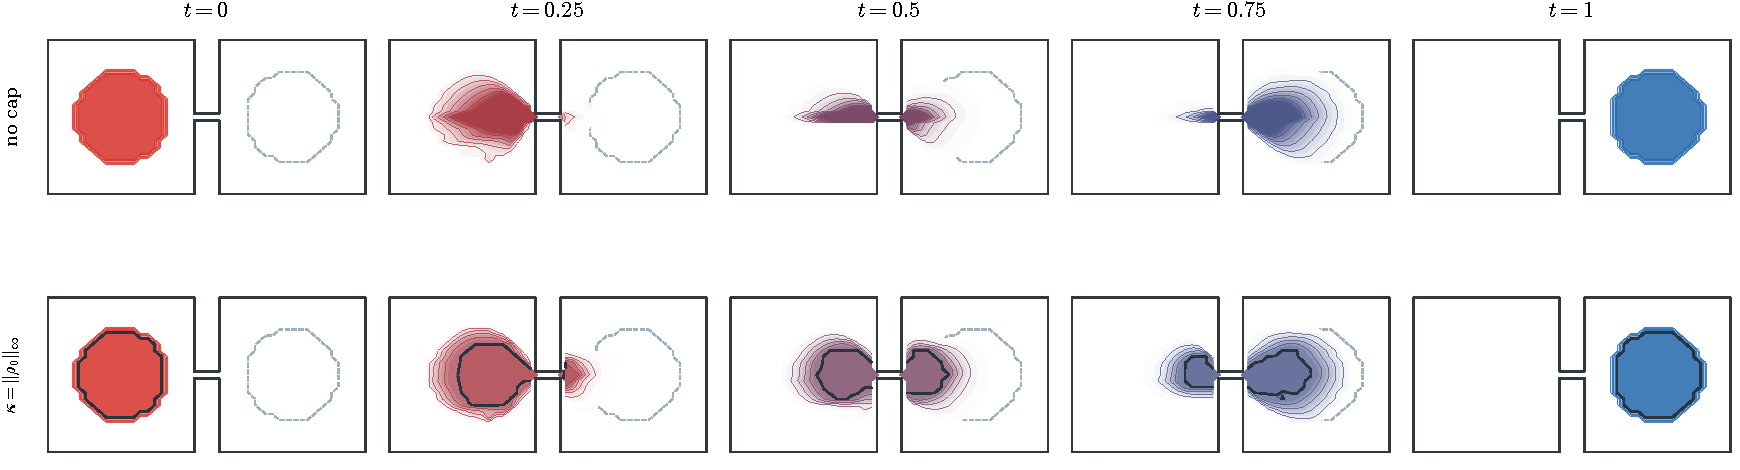
\includegraphics[width=.99\linewidth]{figures/dynamic-variational-mfg-hard-congestion/evolution.pdf}
\caption{\emph{Hard-congestion variational MFG through two communicating rooms.} The bounded two-room domain has impermeable walls and a single narrow doorway. The initial and hard terminal profiles are uniform on mirrored disks; the dashed outlines show the latter, and the five columns advance from red to blue. The top row has no cap and concentrates into a narrow doorway jet. The bottom row imposes $\kappa=\|\rho_0\|_\infty$ everywhere, forcing a broader saturated queue. Dark contours mark regions within $1\%$ of the cap, and both rows use the same density levels.}
\label{fig:dynamic-variational-mfg-hard-congestion}
\end{figure}

\begin{rem}[Scope of the variational reduction]
	A general MFG need not be the optimality system of a global convex functional. The reduction above applies because the coupling is the first variation of the potential $\mathcal C_G$ and the terminal cost is linear, or more generally convex, in the final law. More general nonlocal, non-potential or non-monotone couplings retain the coupled best-response/consistency interpretation but generally fall outside~\eqref{eq-variational-mfg-momentum}.
\end{rem}

\paragraph{Computational consequence.}
\index{augmented Lagrangian}% strictindex
The convexification is not merely formal. After conservative space--time discretization, the objective is a sum of local perspective and congestion terms subject to one affine divergence constraint. Augmented-Lagrangian and primal--dual methods can therefore alternate local proximal updates with the solution of a linear space--time equation, closely paralleling the Benamou--Brenier solver. This route was developed for transport and variational MFGs by Benamou and Carlier~\cite{benamou2015augmented} and is reviewed with numerical examples in~\cite{BenamouCarlierSantambrogio2017}.

The chapter has separated three dynamic transport mechanisms---local advection, nonlocal jumps, and coupled displacement--reaction---and then shown how the local Benamou--Brenier action becomes a convex population game after adding a potential congestion cost. The next chapter uses dynamic transport geometries to turn energies on measures into evolution equations.
